%% This is the ctufit-thesis example file. It is used to produce theses
%% for submission to Czech Technical University, Faculty of Information Technology.
%%
%% This is version 1.6.0, built 18. 9. 2025.
%% 
%% Get the newest version from
%% https://gitlab.fit.cvut.cz/theses-templates/FITthesis-LaTeX
%%
%%
%% Copyright 2024, Tomas Novacek
%% Copyright 2021, Eliska Sestakova and Ondrej Guth
%%
%% This work may be distributed and/or modified under the
%% conditions of the LaTeX Project Public License, either version 1.3
%% of this license or (at your option) any later version.
%% The latest version of this license is in
%%  https://www.latex-project.org/lppl.txt
%% and version 1.3 or later is part of all distributions of LaTeX
%% version 2005/12/01 or later.
%%
%% This work has the LPPL maintenance status `maintained'.
%%
%% The current maintainer of this work is Tomas Novacek (novacto3@fit.cvut.cz).
%% Alternatively, submit bug reports to the tracker at
%% https://gitlab.fit.cvut.cz/theses-templates/FITthesis-LaTeX/issues
%%
%%

% arara: xelatex
% arara: biber
% arara: xelatex
% arara: xelatex

%%%%%%%%%%%%%%%%%%%%%%%%%%%%%%%%%%%%%%%%%
% CLASS OPTIONS
% language: czech/english/slovak
% thesis type: bachelor/master/dissertation/doctoral-report
% electronic (oneside) or printed (twoside), twoside is default
% paragraph - if passed, this optional argument sets paragraphs as the deepest level of headers, styles it, numbers it and adds it to Table of Content. Use with care! Normally, it is considered unwise to use it, since it is too deep.
% colour: bw for black&white OR no option for default colour scheme
%%%%%%%%%%%%%%%%%%%%%%%%%%%%%%%%%%%%%%%%%
\documentclass[czech,bachelor,oneside]{ctufit-thesis}

%%%%%%%%%%%%%%%%%%%%%%%%%%%%%%%%%%
% FILL IN THIS INFORMATION
%%%%%%%%%%%%%%%%%%%%%%%%%%%%%%%%%%
\ctufittitle{Název příkladné závěrečné práce} % replace with the title of your thesis
\ctufitauthorfull{Bc. Žaneta Trošková } % replace with your full name (first name(s) and then family name(s) / surname(s)) including academic degrees
\ctufitauthorsurnames{Trošková} % replace with your surname(s) / family name(s)
\ctufitauthorgivennames{Žaneta} % replace with your first name(s) / given name(s)
\ctufitsupervisor{Ing.\,Milan Dojčinovski,\,Ph.D.} % replace with name of your supervisor/advisor (include academic degrees)
\ctufitdepartment{Katedra softwarového inženýrství} % replace with the department of your defence
\ctufitprogram{Informatika} % replace with your study program
\ctufitspecialisation{Webové inženýrství} % replace with your specialisation
\ctufityear{2026} % replace with the year of your defence
\ctufitdeclarationplace{Praze} % replace with the place where you sign the declaration
\ctufitdeclarationdate{\today} % replace with the date of signature of the declaration
\ctufitabstractCZE{Fill in the abstract of this thesis in Czech. Lorem ipsum dolor sit amet. Class aptent taciti sociosqu ad litora torquent per conubia nostra, per inceptos hymenaeos. Cras pede libero, dapibus nec, pretium sit amet, tempor quis. Sed vel lectus. Donec odio tempus molestie, porttitor ut, iaculis quis, sem. Suspendisse sagittis ultrices augue.}
\ctufitabstractENG{Fill in the abstract of this thesis in English. Lorem ipsum dolor sit amet. Class aptent taciti sociosqu ad litora torquent per conubia nostra, per inceptos hymenaeos. Cras pede libero, dapibus nec, pretium sit amet, tempor quis. Sed vel lectus. Donec odio tempus molestie, porttitor ut, iaculis quis, sem. Suspendisse sagittis ultrices augue.}
\ctufitkeywordsCZE{enter, comma, separated, list, of, keywords, in, CZECH}
\ctufitkeywordsENG{enter, comma, separated, list, of, keywords, in, ENGLISH}
%%%%%%%%%%%%%%%%%%%%%%%%%%%%%%%%%%
% END FILL IN
%%%%%%%%%%%%%%%%%%%%%%%%%%%%%%%%%%

%%%%%%%%%%%%%%%%%%%%%%%%%%%%%%%%%%
% CUSTOMIZATION of this template
% Skip this part or alter it if you know what you are doing.
%%%%%%%%%%%%%%%%%%%%%%%%%%%%%%%%%%

\RequirePackage{iftex}[2020/03/06]
\iftutex % XeLaTeX and LuaLaTeX
    \RequirePackage{ellipsis}[2020/05/22] %ellipsis workaround for XeLaTeX
\else
    \errmessage{Only compilation with XeLaTeX or LuaLaTeX is allowed}
    \stop
\fi

% hyperlinks
\hypersetup{
    pdfpagelayout=TwoPageRight,
    colorlinks=false,
    allcolors=decoration,
    pdfborder={0 0 0.1}
}

% uncomment the following to hide all hyperlinks
%\hypersetup{hidelinks}

% uncomment the following to change the colour of all hyperlinks to CTU blue
%\hypersetup{allbordercolors=decoration}

\RequirePackage{pdfpages}[2020/01/28]

%%%%%%%%%%%%%%%%%%%%%%%%%%%%%%%%%%
% CUSTOMIZATION of this template END
%%%%%%%%%%%%%%%%%%%%%%%%%%%%%%%%%%


%%%%%%%%%%%%%%%%%%%%%%
% PACKAGES SETTINGS
% You may choose to modify this part.
%%%%%%%%%%%%%%%%%%%%%%
\usepackage{dirtree}
\usepackage{lipsum,tikz}
\usepackage[style=iso-numeric]{biblatex}
\addbibresource{text/bib-database.bib}
\usepackage{xurl}
\usepackage{xcolor}
\usepackage{listings} % typesetting of sources

% Define TypeScript language for listings
\lstdefinelanguage{TypeScript}{
  keywords={const, let, var, function, return, if, else, for, while, break, continue, switch, case, default, export, import, from, class, interface, type, extends, implements, public, private, protected, static, async, await, new, this, super, typeof, instanceof, void, null, undefined, true, false},
  keywordstyle=\color{blue}\bfseries,
  ndkeywords={boolean, number, string, any, never, unknown},
  ndkeywordstyle=\color{purple}\bfseries,
  identifierstyle=\color{black},
  sensitive=true,
  comment=[l]{//},
  morecomment=[s]{/*}{*/},
  commentstyle=\color{gray}\ttfamily,
  stringstyle=\color{red}\ttfamily,
  morestring=[b]',
  morestring=[b]",
  morestring=[b]`
}

\lstset{
  basicstyle=\small\ttfamily,
  breaklines=true,
  frame=single,
  numbers=left,
  numberstyle=\tiny\color{gray},
  showstringspaces=false,
  tabsize=2,
  captionpos=b
}

%\usepackage{minted}
\usepackage{csquotes}
\usepackage{pdfx}
\usepackage{datetime} % sometimes helps with CreationDate

%%%%%%%%%%%%%%%%%%%%%%
% PACKAGES SETTINGS END
%%%%%%%%%%%%%%%%%%%%%%

\begin{document}
\frontmatter\frontmatterinit % do not remove these two commands

\thispagestyle{empty}\maketitle\thispagestyle{empty}\cleardoublepage % do not remove these four commands

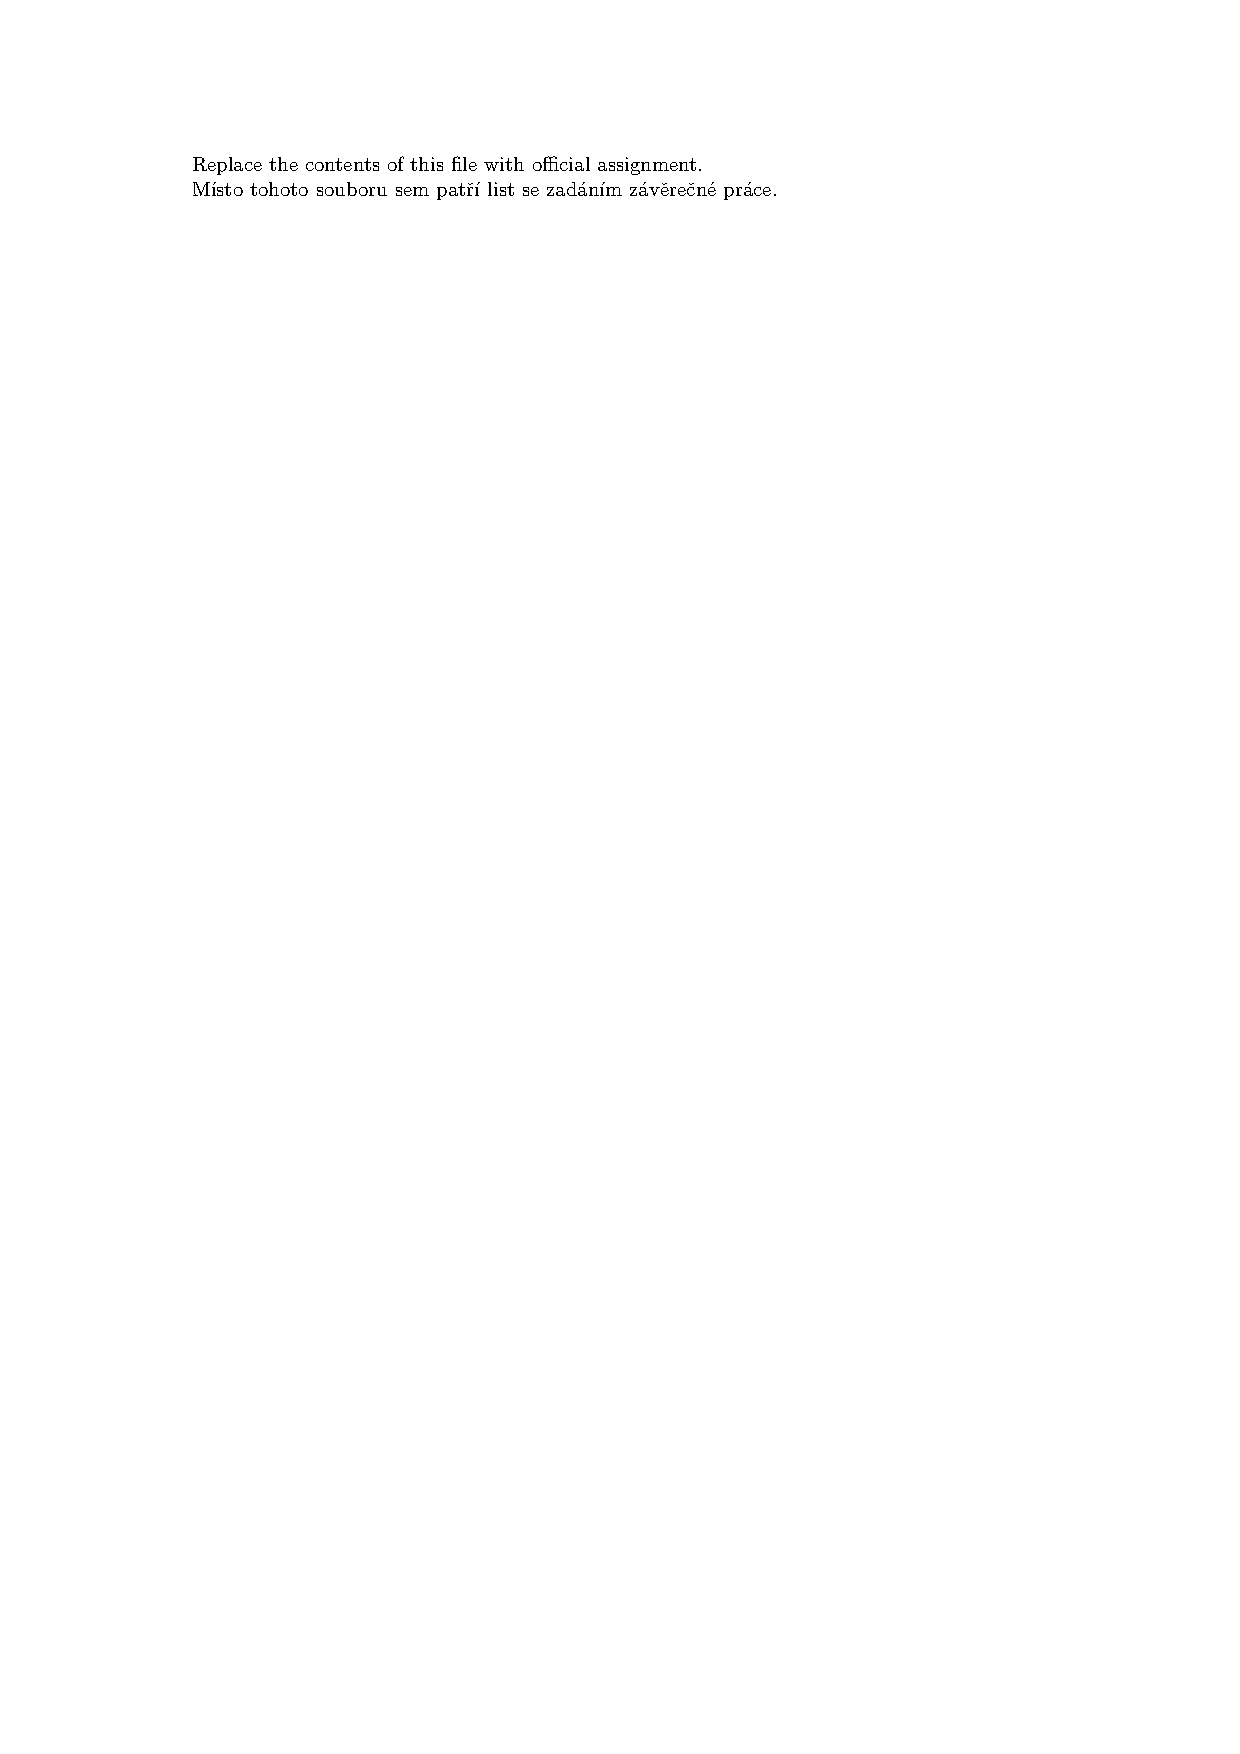
\includepdf[pages={1-}]{example-assignment-include.pdf} % replace this file with your thesis assignment generated from ProjectsFIT

\imprintpage % do not remove this command
\stopTOCentries

%%%%%%%%%%%%%%%%%%%
% ACKNOWLEDGMENT
% FILL IN / MODIFY
% This is a place to thank people for helping you. It is common to thank your supervisor.
%%%%%%%%%%%%%%%%%%%
\begin{acknowledgmentpage}
	Chtěl bych poděkovat především sit amet, consectetuer adipiscing elit. Curabitur sagittis hendrerit ante. Class aptent taciti sociosqu ad litora torquent per conubia nostra, per inceptos hymenaeos. Cras pede libero, dapibus nec, pretium sit amet, tempor quis. Sed vel lectus. Donec odio tempus molestie, porttitor ut, iaculis quis, sem. Suspendisse sagittis ultrices augue.
\end{acknowledgmentpage}
%%%%%%%%%%%%%%%%%%%
% ACKNOWLEDGMENT END
%%%%%%%%%%%%%%%%%%%


%%%%%%%%%%%%%%%%%%%
% DECLARATION
% FILL IN / MODIFY
%%%%%%%%%%%%%%%%%%%
% INSTRUCTIONS
% ENG: choose one of approved texts of the declaration. DO NOT CREATE YOUR OWN. Find the approved texts at https://courses.fit.cvut.cz/SFE/download/index.html#_documents (document Declaration for FT in English)
% CZE/SLO: Vyberte jedno z fakultou schvalenych prohlaseni. NEVKLADEJTE VLASTNI TEXT. Schvalena prohlaseni najdete zde: https://courses.fit.cvut.cz/SZZ/dokumenty/index.html#_dokumenty (prohlášení do ZP)
\begin{declarationpage}
	FILL IN ACCORDING TO THE INSTRUCTIONS. VYPLŇTE V SOULADU S POKYNY. Lorem ipsum dolor sit amet, consectetuer adipiscing elit. Curabitur sagittis hendrerit ante. Class aptent taciti sociosqu ad litora torquent per conubia nostra, per inceptos hymenaeos. Cras pede libero, dapibus nec, pretium sit amet, tempor quis. Sed vel lectus. Donec odio tempus molestie, porttitor ut, iaculis quis, sem. Suspendisse sagittis ultrices augue. Donec ipsum massa, ullamcorper in, auctor et, scelerisque sed, est. In sem justo, commodo ut, suscipit at, pharetra vitae, orci. Pellentesque pretium lectus id turpis.

	Lorem ipsum dolor sit amet, consectetuer adipiscing elit. Curabitur sagittis hendrerit ante. Class aptent taciti sociosqu ad litora torquent per conubia nostra, per inceptos hymenaeos. Cras pede libero, dapibus nec, pretium sit amet, tempor quis. Sed vel lectus. Donec odio tempus molestie, porttitor ut, iaculis quis, sem. Suspendisse sagittis ultrices augue. Donec ipsum massa, ullamcorper in, auctor et, scelerisque sed, est. In sem justo, commodo ut, suscipit at, pharetra vitae, orci. Pellentesque pretium lectus id turpis.
\end{declarationpage}
%%%%%%%%%%%%%%%%%%%
% DECLARATION END
%%%%%%%%%%%%%%%%%%%

% Use one of the two following commands. The first prints abstracts+keywords on two pages, the second puts them on one page (if possible). \printonepageabstract can also accept optional argument that specifies a vertical space before both abstracts (the default is 18 mm).
\printtwopageabstract
%\printonepageabstract 

%%%%%%%%%%%%%%%%%%%
% SUMMARY
% FILL IN / MODIFY
% OR REMOVE ENTIRELY (upon agreement with your supervisor)
% (appropriate to remove in most theses)
%%%%%%%%%%%%%%%%%%%
% \begin{summarypage}
% \section*{Summary section}
% 
% \lipsum[1][1-8]
% 
% \section*{Summary section}
% 
% \lipsum[2][1-6]
% 
% \section*{Summary section}
% 
% \lipsum[3]
% 
% \section*{Summary section}
% 
% \lipsum[2]
% 
% \section*{Summary section}
% 
% \lipsum[1][1-8] Lorem lorem lorem.
% \end{summarypage}
%%%%%%%%%%%%%%%%%%%
% SUMMARY END
%%%%%%%%%%%%%%%%%%%

\tableofcontents % do not remove this command
%%%%%%%%%%%%%%%%%%%%%%
% list of other contents: figures, tables, code listings, algorithms, etc.
% add/remove commands accordingly
%%%%%%%%%%%%%%%%%%%%%%
\listoffigures % list of figures
\begingroup
\let\clearpage\relax
\listoftables % list of tables. Remove if you do not have any.
\thectufitlistingscommand{} % list of code listings. Remove if you do not have any.
\thectufitlistofalgorithmscommand{} % list of algorithm pseudocodes defined using the algorithm package.
\endgroup
%%%%%%%%%%%%%%%%%%%%%%
% list of other contents END
%%%%%%%%%%%%%%%%%%%%%%

%%%%%%%%%%%%%%%%%%%
% ABBREVIATIONS
% FILL IN / MODIFY
% OR REMOVE ENTIRELY
% List the abbreviations in lexicography order.
%%%%%%%%%%%%%%%%%%%
\chapter{\thectufitabbreviationlabel}

\begin{tabular}{rl}
	DFA   & Deterministic Finite Automaton                 \\
	FA    & Finite Automaton                               \\
	LPS   & Labelled Prüfer Sequence                       \\
	NFA   & Nondeterministic Finite Automaton              \\
	NPS   & Numbered Prüfer Sequence                       \\
	XML   & Extensible Markup Language                     \\
	XPath & XML Path Language                              \\
	XSLT  & eXtensible Stylesheet Language Transformations \\
	W3C   & World Wide Web Consortium
\end{tabular}
%%%%%%%%%%%%%%%%%%%
% ABBREVIATIONS END
%%%%%%%%%%%%%%%%%%%
\resumeTOCentries
\mainmatter\mainmatterinit % do not remove these two commands
%%%%%%%%%%%%%%%%%%%
% THE THESIS
% MODIFY ANYTHING BELOW THIS LINE
%%%%%%%%%%%%%%%%%%%

% Do not forget to include Introduction
%---------------------------------------------------------------
\chapter{Úvod}
% uncomment the following line to create an unnumbered chapter
%\chapter*{Introduction}\addcontentsline{toc}{chapter}{Introduction}\markboth{Introduction}{Introduction}
%---------------------------------------------------------------
\setcounter{page}{1}

% The following environment can be used as a mini-introduction for a chapter. Use that any way it pleases you (or comment it out). It can contain, for instance, a summary of the chapter. Or, there can be a quotation.
% \begin{chapterabstract}
% 	\lipsum[1]
% \end{chapterabstract}

%%%%%%%%%%%%%%%%%%%%%%%%%%%%%%%%%
% alternative using package minted for source highlighting
% package minted requires execution with `-shell-escape'
% e.g., `xelatex -shell-escape ctufit-thesis.tex'
% \begin{listing}
% \begin{minted}{C}
%     #include<stdio.h>
%     #include<iostream>
%     // A comment
%     int main(void)
%     {
%         printf("Hello World\n");
%         return 0;
%     }
% \end{minted}
% \caption{Zbytečný kód}\label{list:8-6}
% \end{listing}
% %%%%%%%%%%%%%%%%%%%%%%%%%%%%%%%%%

Společenské tance (často označované anglickým termínem \emph{social dance}) jsou tance, které se tančí především za účelem zábavy a společenské interakce. V~posledních letech nabývají na popularitě a s tím roste i množství tanečních kurzů, workshopů a akcí. Tanců je několik, avšak s ohledem na cílovou skupinu se tato práce zaměřuje na salsu, bachatu a zouk.

S narůstajícím počtem událostí se sice rozšiřují možnosti pro taneční komunitu, zároveň je ale stále náročnější se v této nabídce přehledně orientovat. Pro začínající tanečníky bývá obtížné zjistit, kde a kdy se konají vhodné akce a jaké jsou jejich podmínky (úroveň, typ události, cena či lokalita). Zkušenější tanečníci naopak často hledají konkrétnější akce podle stylu nebo místa a potřebují rychle porovnat více možností. Z pohledu organizátorů je klíčová především přehledná správa událostí a registrací účastníků.

V praxi jsou informace o událostech často rozptýlené napříč více kanály. Část organizátorů zveřejňuje akce na webových stránkách nebo v kalendářích tanečních škol, významná část komunikace probíhá na sociálních sítích (typicky Facebook a Instagram) a registrace bývají řešeny externě, například přes Google Formuláře či zprávy. Tato roztříštěnost vede k tomu, že tanečníci musí události složitě dohledávat, a i po registraci mohou postrádat jasné potvrzení nebo přehled o svých přihláškách. Organizátorům naopak chybí jednotné místo pro prezentaci akcí a nástroje pro přehlednou administraci účastníků.

Tuto problematiku řeší tato diplomová práce, jejímž tématem je návrh a implementace webové aplikace pro správu společenských tanečních akcí a kurzů, která by spojovala tanečníky a organizátory. Nápad na téma vznikl z osobního zájmu autorky o společenské tance a z pozorování, že existuje mezera na trhu pro platformu, která by poskytla centralizovaný a přehledný přístup k událostem i jejich správě.

Cílem této práce je navrhnout, implementovat a vhodně otestovat webovou aplikaci pro správu společenských tanečních akcí a kurzů, která tanečníkům usnadní vyhledávání událostí a organizátorům umožní přehlednou správu akcí a registrací účastníků.
\chapter{Social dance}
% mini introduction about the chapter
\begin{chapterabstract}
	Následující kapitolu uvedu do problematiky společenských tanců, vysvětlím co to jsou společenské tance, jaké druhy společenských tanců existují a jaké jsou jejich charakteristiky. Následně zanalyzuji jaké nástroje a technologie jsou využívány uživateli pro vyhledávání kurzů a akcích spojenými s těmito tanci. Nakonec popíši motivaci pro vytvoření aplikace, která by uživatelům to vyhledávání usnadnila. 
\end{chapterabstract}
\section{Co jsou to společenské tance}
Společenské tance (více známé jako nepřekládané "social dance") jsou tance, které se tančí především kvůli zábavě a společenské interakci mezi lidmi, na rozdíl od jiných forem tanců, které se zaměřují na soutěžení. Avšak je důležité poznamenat, že některé 
taneční akce nebo festivaly začali zahrnovat i možnost zúčastnit se soutěží. Soutěže ovšem bývají jinak postavené než klasické taneční soutěže, protože partneři bývají náhodně přiřazeni. Tudíž tanečníci nemají možnost si s partnerem předem nacvičit choreografii, ale musí se spolehnout na své schopnosti improvizace a komunikace během tance.
\cite{socialDance:about}

Společenské tance bývají nejčastěji párové tance, kde partneři spolu komunikují prostřednictvím pohybů a vedení. Jeden z partnerů obvykle bývá označován jako "vedoucí" (leader) a druhý jako "následující" (follower). Leader vede tanec a určuje směr a styl pohybu, zatímco follower reaguje na jeho vedení a doplňuje tanec svými vlastními pohyby. Co je na tanci zajímavé, je to že tyto tance se tancují většinou improvizovaně, což znamená, že neexistují pevně stanovené kroky nebo choreografie, které by museli tanečníci dodržovat. Místo toho leader vymýšlí kroky a pohyby na místě a pomocí správného vedení umožňuje followerovi správně reagovat. 
 \cite{socialDance:about}

\section{Druhy společenských tanců}
Existuje mnoho druhů společenských tanců, které se liší svým stylem, rytmem a kulturou, ze které pocházejí. Já jsem se rozhodla pro účely mé diplomové práce se zaměřit na druhy tanců se kterými se nejvíce setkávám v mé taneční komunitě. Jedná se o následující tance:
\begin{itemize}
    \item Salsa
    \item Bachata
    \item Zouk
\end{itemize}
V následující sekci popíši charakteristiky těchto tanců. Samozřejmě můžeme zmínit i další tance, se kterými se člověk taky může setkat, jako například Kizomba, Swing, Reggaeton a další, ale pro účely této práce jsem se rozhodla zaměřit pouze na ty tři, které jsem zmínila výše, protože jsou mi nejvíce blízské a setkávám se s nimi nejčastěji.

Také jsem se setkala s tím, že se taneční styly kombinují dohromady, tomuto pojmu se říká "fusion". \cite{centrumtance_dance_fusion}

Nejvíce jsem se za poslední dobu setkala s trendem, kde se kombinuje bachata s zoukem, tento styl se nazývá "bachazouk". TODO

\subsection{Salsa}
Je latinsko-americký tanec s kubánskými kořeny vyznačující se rychlým tempem, energickými pohyby a výraznou rytmikou. Tanec působí živě a radostně, což z něj činí vhodnou volbu pro společenské události a taneční večery. \cite{socialDance:salsa}

Tento tanec vznikl zhruba ve 30 letech 20. století na Kubě a později se rozšířil do dalších částí Latinské Ameriky. Salsa se následně kvůli migraci rozšířila i do Spojených států, kde byla braná jako populární zábava. Díky tomuto se salsa různě proměňovala a vyvíjela, což vedlo k vytvoření různých stylů salsy. \cite{socialDance:salsa:history}

Salsa se většinou tančí na hudbu ve čtyřčtvrtečním taktu na doby 1, 2, 3 a 5, 6, 7, přičemž doba 4 a 8 jsou pauzy (avšak některé styly salsy mohou mít odlišné rytmus jako například New York salsa, která se tančí na doby 2, 3, 4 a 6, 7, 8). \cite{socialDance:salsa:rhythm}

Z mé zkušenosti je salsa často na akcích ruku v ruce s bachatou, například v jedné místnosti se tančí salsa a v druhé místnosti se tančí bachata. Také se dějí tzv. SBK party, což znamená, že se tančí salsa, bachata a kizomba. 

\subsection{Bachata}
Bachat je tanec pocházející z Dominikánské republiky, který je rozšířený po celém světě. 
Je známá především jako sensuální tanec. V tomto tanci se tančí sekvence kroků na 8 dob, v originálu se tančí do čtverce, ale v západním světě se začalo do strany, což je jednodušší. V obou případech se tančí 3 kroky a poté následuje tzv. "tap", což je 
krok, kdy se noha zvedne a poklepe o zem (často doprovázená bokem do strany), ale nedělá se krok. \cite{incognitodance_what_is_bachata}

Bachata se dělí na několik stylů, přičemž tanečníci často kombinují různé styly dohromady. Chtěla bych zmínit ty nejběžnější styly, které se tančí v mé komunitě, jako například \cite{jtdancestudio_bachata_styles}:
\begin{itemize}
    \item Dominikánská bachata - tento styl je ve své původní podobě jednou z nejjednodušších, ale zároveň nejživějších forem tohoto tance. Tento styl se vyznačuje hravým footworkem a pohybem boků do strany podle rytmu hudby. Tento styl neobsahuje komplikované figury, což ho činí vynikajícím pro začátečníky.
    \item Bachata Moderna - nazývána také jako "moderní bachata" je styl, který mixuje tradiční bachatu s jinými tanečními styly, jako je například salsa. Tento styl se především vyznačuje většími pohyby, dynamičtější projev a rychlé otočky. Také obsahuje více záklonů než bychom třeba shledali u původní bachaty.
    \item Sensual - tento styl vznikl ve Španělsku díky tanečníkům Korke Escalona a Judith Cordero za cílem přidat do bachaty více výrazů a emocí. Tento styl kombinuje prvky moderní bachaty s kroky brazilského zouku. Typickými prvky toho stylu jsou vlnící se pohyby těla a izolace (oddělené pohyby různých částí těla). Tanečníci obvykle tančí blízko sebe a pohybují se jako jeden celek, což navozuje emotivní a romantickou atmosféru.
\end{itemize}

\subsection{Zouk}
Je partnerský tanec, pocházející z Brazílie. Tento tanec vznikl v počátcích 90. let 20. století a byl ovlivněn karabskou zouk hudbou a tancem lambada. Během let se zouk vyvinul do několika stylů, přičemž se dá tančit nejenom na zouk hudbu, ale i například na hip hop, R\&B, pop hudbu a další. Zouk se obecně vyznačuje vedením pomocí celého těla, nakloněné (říká se off-axis) pozice, otočky a náklony partnerky. Charakteristické pro zouk jsou také pohyby hlavy partnerky (říká se jim tzv. “hair movement”), které vznikají nakláněním followera při vedení. Tyto pohyby jsou dle mého názoru jedním z nejzajímavějších aspektů tohoto tance a zároveň i jedním z nejtěžších, protože vyžadují velkou kontrolu nad tělem a správné vedení. Zároveň jsem si všimla, že tyto figury se začaly objevovat i v bachtě, díky tomu, jak vypadají dobře. \cite{zoukminneapolis_brazilian_zouk}



\section{Cesta tanečníka ve světě společenských tanců}
Lidé se do světa společenských tanců často dostávají z různých důvodů. Z mojí zkušenosti nejčastěji prostřednictvím přátel, kteří již tančí, sociálních sítí, kde jsou propagovány taneční workshopy a kurzy, nebo prostřednictvím videí na platformách jako je YouTube, kde lidé objevují různé taneční styly a chtějí se je naučit.

Většinou si člověk vybere konkrétní tanec, který ho zaujal, a začne hledat kurzy nebo taneční školy, které tento tanec nabízejí. Tudíž prvním krokem bývá nalezení vhodného kurzu.
Po pár lekcích tanečníci často začínají navštěvovat taneční akce, kde mohou tančit s různými partnery a zlepšovat své dovednosti v reálném prostředí. Na kurz člověk nemusí přijít v páru, protože se na lekcích partneři většinou střídají. Občas jsem se i setkala s tím, že kurz bývá koncipován tak, že nejprve proběhne výuková hodina/workshop, a poté následuje 
party, při které lidé procvičují co se naučili a improvizují. Zkušenější tanečníci se mohou účastnit různých tanečních festivalů, v rámci nichž probíhají workshopy a taneční večery. Některé taneční školy nebo organizace nabízejí i sérii workshopů anebo hodin v rámci kurzu, na které se mohou tanečníci jednotlivě hlásit a tudíž si mohou vybrat konkrétní lekce, které je zajímají anebo se jim hodí do časové kapacity, místo toho, aby se hlásili na celý kurz.
Velkým zážitkem dle mého názoru je i cestování na taneční akce do jiných měst nebo zemí, kde mohou tanečníci poznat nové lidi a kultury prostřednictvím tance. \cite{socialDance:about}

\section{Existující prostředky pro vyhledávání událostí}
V předchozí sekci jsem popsala jak se tanečníci dostávají do světa společenských tanců a jaké události mohou navštěvovat. V této sekci zanalyzuji jaké nástroje a technologie jsou využívány uživateli pro vyhledávání kurzů a akcích spojenými s těmito tanci. Při tvorbě této analýzy jsem vycházela z vlastních zkušeností s vyhledáváním kurzů a akcí, zejména v oblasti bachaty v Praze, jelikož dlouhodobě na tyto akce docházím a jsem schopna lépe zhodnotit dostupné nástroje. Tato analýza byla zároveň konzultována s dalšími tanečníky působícími v této komunitě, kteří poskytli podněty vedoucí k jejímu zlepšení.

\subsection{Webové stránky tanečních škol}
Webové stránky byly pro mě prvním místem, kde jsem hledala informace o kurzech a akcích. Většina tanečních škol má své vlastní webové stránky, kde zveřejňují informace o nabízených kurzech, termínech, cenách a dalších detailech. Tyto stránky často obsahují i kalendář akcí, kde jsou uvedeny nadcházející taneční večery a workshopy. Nicméně, nevýhodou je, že uživatel
musí procházet webové stránky tanečních škol jednotlivě a stranou si poznamenávat informace o kurzech, což může být časově náročné a únavné. Navíc je možné, že nějaké organizace/spolky nemají vlastní webové stránky, ale působí jen na sociálních sítích, tudíž na ně uživatel nemůže narazit na webu.

Existují i stránky, které agregují informace z více tanečních škol a spolků. Některé tyto stránky jsou koncipované tak, že abyste mohli přidat událost, musíte uzavřít spolupráci s danou stránkou, což často zahrnuje i poplatek anebo si berou provizi z prodeje vstupenek. Toto může být pro některé organizace odrazující faktor, což vede k tomu, že událostí na těchto stránkách není tak hojný počet. Jedna z příkladů těchto stránek je go \& dance, která se hlavně zaměřuje na propagaci velkolepých festivalů a kongresů. Tyto akce bývají v řádech stovek eur, což je poměrně drahé v porovnáním kolik stojí běžné kurzy a taneční večery. Stránka má hezký design a je přehledná, avšak pokud se snažím najít akce konající se v Praze, tak mi stránka vrátí i akce konající se v jiných městech. Toto je pro mě poměrně frustrující, protože musím procházet všechny akce a hledat ty, které se konají v Praze.

Jako další příklad jsem nalezla stránku tanci.cz, která cílila na kurzy a události pořádané v ČR, avšak tato stránka se jeví jako nefunkční a nenalézá mi žádné kurzy.
%% mam uvadet obrazkama priklady?
\subsection{Sociální sítě}
Sociální sítě jsou dle mého pozorování nejběžnějším prostředkem k vyhledávání nadcházejících tanečních akcích a zároveň i slouží jako platforma pro komunikaci mezi tanečníky a organizátory. Dle mého pozorování je nejčastější platformou pro tento účel Facebook. 

Na facebooku organizátoři vytvářejí události, kde zveřejňují informace o nadcházejících akcích, jako jsou termíny, místa konání, ceny a další detaily. Většina z nich pro registrace používá buď že napíšete zprávu organizátorovi anebo google formuláře. Registrace bývá občas trochu chaotická, protože vyplníte například google formulář, ale nemáte jistotu, že organizátor váš zájem o účast zaznamenal, protože vám nepřijde žádné potvrzení o registraci. Také se stává, že tím jak je organizování dáno přes zprávy, tak se populárním organizátorům špatně udržují čekací listiny. To může vést k demotivaci lidí, kteří se snaží do kurzu dostat.  

Uživatelé mohou události na facebooku sledovat, přihlásit se na ně a sdílet je se svými přáteli. Facebook také umožňuje organizátorům cíleně propagovat své události prostřednictvím placených reklam, což zvyšuje jejich viditelnost a dosah. Nicméně, nevýhodou je, že pokud sociální síť nevyhodnotí, že by daná akce byla pro uživatele relevantní, nezobrazí ji. Tím uživatel může přijít o informace o akcích, které by ho mohly zajímat.  

Uživatelé musí procházet různé skupiny, stránky a události, aby našli relevantní informace o nadcházejících akcích, což může být časově náročné a frustrující. Je také docela těžké dohledat akci co v případě hledání třeba klíčového slova "bachata" umístěného v Praze, v názvu bachata nemá. Pak mi facebook akci nenabídne, ale nabízí mi akce, které mají v názvu "bachata", ale nejsou umístěné v Praze.
Z mé zkušenosti velmi pomohlo, když jsem se na facebooku propojila s tanečníky, protože mi to umožnilo vidět události, o které mají zájem a tímto se stalo pro mne jednodušší akce dohledávat. 

Další sociální sítí, která se využívá pro tento účel, je Instagram. Na Instagramu organizátoři často sdílejí informace o nadcházejících akcích prostřednictvím příspěvků a příběhů. Uživatelé mohou sledovat účty organizátorů a získávat informace o nadcházejících akcích. Nicméně je zde ještě horší vyhledávání akcí a spíše se instagram využívá pro propagaci akcí a komunikaci s uživateli, než pro samotné vyhledávání.

Po té jsou tu i další platformy jako například Whatsapp, kde se často vytvářejí skupiny pro tanečníky, kteří spolu komunikují a sdílejí informace o nadcházejících akcích. Tyto skupiny jsou často uzavřené a přístupné pouze pro členy, což může být nevýhodou pro nové tanečníky, kteří se snaží najít informace o akcích.

Tyto sociální sítě jsou velmi užitečné pro komunikaci a propagaci akcí, ale nejsou ideální pro samotné vyhledávání, protože sociální sítě jsou zaměřené obecně na komunikaci a sdílení, a ne na organizaci a vyhledávání tanečních akcí. další problémem se kterým se potýkám je rozptýlenost informací.
Některé akce jsou propagovány pouze na facebooku, jiné pouze na instagramu a další pouze prostřednictvím whatsappových skupin. Tudíž dochází k tomu, že uživatel musí procházet různé platformy, aby našel informaci, kterou někdy viděl, ale už si nepamatuje kde. Dále tím, že jedna akce je na více platformách, tak se může stát, že jsou informace o ní nekonzistentní. Například se mi jednou stalo, že jsem se přihlásila na akci na facebooku a později jsem se přidala do whatsappové skupiny, která souvisela s touto akcí, ale účast v ní nebyla povinná pro účast na akci. Po té došlo ke změně času konání akce, ale já jsem se o této změně dozvěděla až v den konání akce, ale informace byla zprostředkována pouze prostřednictvím whatsappové skupiny, ale ne na facebooku. Tím že většina lidí o akci věděla pouze z facebooku, tak se stalo, že mnoho lidí se na akci dostavilo pozdě a nemohli se tak zúčastnit naplánovaného workshopu. dalším problémem je, že uživatel kromě svých přátel nevidí kdo se na akci přihlásil a jaký je poměr mezi leadery a followery.

\subsection{Mobilní aplikace}
Mobilních aplikací, které by zahrnovali různé taneční akce, je poměrně málo. Při prohlížení jednotlivých aplikací jsem narážela na problém, že neobsahují skoro žádné akce a jeví se jako poměrně neaktivní. Poté mi jeden známý doporučil aplikaci "Only Dance", která se nejenom zaměřuje na taneční akce ale také funguje jako sociální síť pro tanečníky. Tato aplikace má poměrně hezký design a nabízí i funkcionality jako možnost vytvářet spojení mezi tanečníky nebo psát příspěvky, které celá komunita může vidět. Nicméně, nevýhodou je, že aplikace obsahuje pouze možnost přidat reakci na akci, že plánuju jít anebo že se mi akce líbí, ale neobsahuje možnost rozlišit role pro akce, kde by to bylo relevantní. Také nemohu vidět kdo na akci jde, pokud uživatele nemám ve spojení. Dále mi přijde škoda, že uživatel nemůže přidávat videa na profil, určitě by to usnadnilo hledání tanečního partnera. Co mě na aplikaci nepříjemně překvapilo je, že když se akce zruší, tak ji aplikace smaže ale neoznačí ji jako zrušenou, což může být pro uživatele matoucí, protože s akcí již počítal a najednou se mu ztratí z přehledu, aniž by věděl, že se akce zrušila.

\subsection{Shrnutí - motivace pro vytvoření nové aplikace}
V předchozích sekcích jsem popsala různé nástroje a technologie, které jsou využívány pro vyhledávání kurzů a akcí spojenými se společenskými tanci. Z mého pohledu je zřejmé, že existuje několik problémů, které uživatelé mohou zažít při hledání těchto informací. Tyto problémy zahrnují rozptýlenost informací, nekonzistentní informace o akcích, nedostatek přehledu o tom, kdo se na akci přihlásil a zda uživatelova akce vedla k úspěšné registraci.
\chapter{Analýza}
\begin{chapterabstract}
    Tato kapitola se zabývá specifikací požadavků na budoucí aplikaci, formulovaných na základě zjištění z předchozí kapitoly. Následně bude rozpracován návrh systému, na jehož základě budou zvoleny vhodné technologie a postupy.
\end{chapterabstract}

\section{Požadavky}
Požadavky jsou důležitou částí vývoje softwaru, protože definují, co má systém dělat a jaké funkce by měl poskytovat uživatelům. Požadavky jsem definovala pomocí MOSCoW metody, která rozděluje požadavky do čtyř kategorií: Must have (musí mít), Should have (mělo by mít), Could have (mohlo by mít) a Won't have (nebude mít). Metodu vytvořil D. Richardson při práci v Oracle za účelem pomoci prioritizovat požadavky pro vývoj softwaru.\cite{moscow:definition}

Tato metoda mi pomohla určit priority jednotlivých požadavků a zaměřit se na ty nejdůležitější funkce pro první verzi aplikace. V následujících podsekcích rozdělím požadavky podle této metodiky a ke každému požadavku přidám popis jeho významu a důležitosti pro budoucí aplikaci.

U každého požadavku jsem rozhodla, zda se jedná o funkční nebo nefunkční požadavek. Funkční požadavky – označené symbolem F před názvem požadavku – popisují konkrétní funkce a chování systému (např. co se má stát po tom co uživatel klikne na tlačítko). Nefunkční požadavky – označené symbolem N před názvem požadavku – specifikují vlastnosti systému (např. zda má být aplikace responzivní nebo jak rychle má zpracovávat transakce). \cite{nonFunctionalVsFunctional:definition}

Veškeré požadavky byly tvořeny na základě konzultací s taneční komunitou, analýzy stávajících řešení a mých vlastních zkušeností, jakožto člověka, který se aktivně účastní tanečních akcí a setkává se s problémy, které způsobují frustraci u tanečníků a organizátorů. Tyto požadavky jsou navrženy tak, aby řešily konkrétní problémy a zlepšovaly celkovou zkušenost s hledáním a organizací tanečních akcí.

\subsection{Must have (musí mít)}
Tyto požadavky jsou nezbytné pro základní funkčnost aplikace. Bez nich nedává nasazení aplikace smysl. Tudíž se jedná o požadavky, na které budu klást větší důraz a dávat jim nejvyšší prioritu při vývoji.\cite{moscow:definition}
\subsubsection{Zobrazení nadcházejících akcí}
Tento požadavek je klíčový pro hlavní účel aplikace, kterým je usnadnit uživatelům vyhledávání tanečních akcí. Aplikace musí být schopna zobrazit seznam nadcházejících akcí spolu s jejich základními informacemi jako:
\begin{itemize}
    \item Název akce
    \item Jméno organizátora
    \item Datum a čas
    \item Místo konání
    \item Cena pokud je uvedena
    \item Tagy přibližující informace o akci, jako je typ tance, úroveň obtížnosti, zda se jedná o kurz, workshop nebo party a další relevantní informace.
    \item počet přihlášených účastníků a počet uživatelů kteří mají o akci zájem
    \item Možnost zobrazit detailní informace o akci
\end{itemize}
Pokud uživatel není organizátor, má navíc možnost se na akci přihlásit anebo ji označit že ho zajímá. Události se navíc vrací po stránkách, aby nedocházelo k zbytečnému načítání velkého množství dat najednou, což by mohlo zpomalit aplikaci.

Tento požadavek je nezbytný, umožní uživatelům snadno najít a prohlédnout si nadcházející taneční akce, aniž by museli jak je to například na facebooku, hledat akce pomocí klíčových slov anebo doufat že se jim akce zobrazí v jejich feedu na základě reakce jejich přátel.

\subsubsection{Filtrování nadcházejících akcí}
Aplikace umožní uživatelům filtrovat nadcházející akce podle různých kritérií, jako jsou:
\begin{itemize}
    \item Název akce
    \item Typ tance (swing, salsa, tango, atd.)
    \item Typ akce (kurz, workshop, party)
    \item Lokalita -filtrování na úrovni města nebo státu
\end{itemize}
Tento požadavek je velmi důležitý, protože umožní uživatelům vyhledávat akce lépe než popsané aplikace popsané v předchozí kapitole. Vyfiltrované události se také budou vracet po stránkách jak je to popsáno v předchozím požadavku.

Tohle mě jako potencionálnímu uživateli například umožní odfiltrovat akce, které se konají pro mě v nedostupné lokalitě anebo akce které jsou zaměřené na jiný taneční styl než ten který preferuji.

\subsubsection{Přihlášení uživatele pomocí Google účtu}
Aplikace musí umožnit uživatelům přihlásit se pomocí svého Google účtu, což zjednoduší proces registrace a přihlášení, a zároveň umožní využít funkce spojené s Google službami, jako je například integrace s Google Forms. Zároveň nám bude poskytnuto jméno a email uživatele, což pro uživatele bude přívětivější mít tyto informace předvyplněné na svém profilu.

\subsubsection{Odhlášení uživatele pomocí Google účtu}
Aplikace musí umožnit uživatelům odhlásit se z aplikace, aby měli například možnost na stejném zařízení používat více účtů. 

\subsubsection{Detail události}
Přihlášený uživatel by měl mít možnost zobrazit detailní informace o události. Tyto informace by měly zahrnovat:
\begin{itemize}
    \item základní informace o akci (název, datum a čas, místo konání, cena, odkaz na facebookovou událost)
    \item popisek akce
    \item informace o organizátorovi (jméno, odkaz na profil)
    \item informace o přihlášených účastnících (počet přihlášených, počet uživatelů kteří mají o akci zájem, popřípadě v jakých rolích jsou uživatelé zastoupeni (leader, follower))
    \item tagy přibližující informace o akci, jako je typ tance, úroveň obtížnosti, zda se jedná o kurz, workshop nebo party a další relevantní informace.
\end{itemize}

Požadavek byl sepsán na základě konzultací s tanečníky, kde jsme diskutovali, jaké informace bychom uvítali u detailu akce, abychom se mohli lépe rozhodnout, zda se na akci přihlásit nebo ne. Opakovaně se mi dostávalo odpovědi, že by bylo užitečné mít informace o tom, kolik lidí se již přihlásilo a kolik lidí má o akci zájem, protože to může být indikátor kvality akce (čím více lidí se přihlásí tím více mám možnost například v případě párového tance ozkoušet různé partnery a akci si tím více užít). 

\subsubsection{Přihlášený uživatel může přidávat vlastní akce}
Přihlášený uživatel by měl mít možnost přidávat vlastní taneční akce do aplikace, což umožní komunitě sdílet informace o různých událostech. Přidání akce je proces, který si klade za cíl strukturovaně uživateli umožnit zadat v přehledném formuláři všechny potřebné informace o akci nezbytné pro její zveřejnění v aplikaci. Formulář organizátorovi poskytuje rozhraní jehož výsledkem bude událost s dostatečnou informační hodnotou pro potencionální účastníky. 

Mezi tyto informace patří:
\begin{itemize}
    \item Název akce
    \item Datum a čas
    \item Místo konání
    \item Cena pokud je uvedena a měna ve které je cena uvedena
    \item Popisek akce
    \item Informace o akci (typ tance, úroveň obtížnosti, druh události)
    \item kapacita akce 
    \item odkaz na facebookovou událost (pokud existuje) - to umožní uživatelům zkontrolovat další informace o akci, které nejsou uvedeny v aplikaci, a zároveň umožní organizátorům snadno propojit svou akci s již existující facebookovou událostí.
\end{itemize}
Uvedené informace o akci byli sestaveny po diskuzích s různými organizátory (ať už se jedná o lektory anebo lidi kteří organizují taneční večírky). Zároveň jsem se inspirovala informacemi, které jsou běžně uváděny v popiscích akcí na facebooku nebo na webových stránkách organizátorů.

Formulář s informacemi bude rozdělen do několika kroků, aby se uživatelé necítili zahlceni množstvím informací, které musí zadat.
Vzhledem k tomu, že organizátor nemusí mít v okamžiku vytváření události k dispozici všechny potřebné informace, případně ji ještě nemusí chtít zveřejnit nebo si přeje nejprve zkontrolovat výslednou podobu detailu akce, tak odeslání formuláře nebude mít za následek okamžité zveřejnění akce v aplikaci. Místo toho se vytvoří koncept události, který bude organizátorovi přístupný pro další úpravy a doplnění informací.
Organizátor bude mít možnost kdykoliv se vrátit k úpravě konceptu a doplnění informací o akci, než ji zveřejní.

\subsubsection{Registrace na událost}
Tento požadavek umožní uživatelům přihlásit se na události přímo prostřednictvím aplikace, což usnadní organizátorům správu registrací a účastníkům jednoduchý způsob, jak se zúčastnit akcí. Tento požadavek je klíčový pro hlavní účel aplikace, kterým je správa registrací na taneční akce.

Aplikace bude umožňovat 3 následné možnosti jak se uživatel bude přihlašovat na akci:
\begin{itemize}
    \item Otevřená registrace - každý se může přihlásit bez omezení do kapacity akce
    \item Párová registrace - každý se může přihlásit do kapacity akce, ale musí uvést zda je leader nebo follower
    \item Registrace pomocí Google formuláře - organizátor může propojit Google formulář pro registraci účastníků přímo s událostí v aplikaci, což by usnadnilo správu registrací.
\end{itemize} 
Tyto možnosti publikace jsou pro organizátory velmi vítané, protože umožní jak např. registraci pro ladies styling workshop, kde je obvykle omezená kapacita a není potřeba uvádět zda je účastník leader nebo follower, tak i pro párové akce, kde je důležité mít přehled o počtu leaderů a followerů. 
A jelikož je google formulář jedním z častějších nástrojů pro registraci účastníků, tak možnost propojení s google formulářem je pro organizátory velmi vítaná.

\subsubsection{Organizátor může publikovat akci}
Po vytvoření konceptu akce bude organizátor mít možnost ji publikovat, což znamená, že se akce stane viditelnou pro všechny uživatele aplikace. Tento krok umožní organizátorovi nastavit jakým způsobem chce registrovat účastníky (vybrat jednu z možností popsaných v předchozím požadavku) a zároveň zvolit další nastavení přihlašování, jako je například možnost schvalovat registrace účastníků manuálně.

\subsubsection{Organizátor může upravovat akci}
Tento požadavek umožní organizátorům upravovat informace o své akci i po jejím zveřejnění, což je důležité pro případ, že se změní nějaké detaily akce nebo pokud organizátor zapomněl uvést nějakou důležitou informaci při vytváření akce.

Dle mých pozorování je běžné, že se mění čas anebo místo konání akce, případně se doplňují informace o programu, které předtím nebyly k dispozici.

\subsubsection{Přihlášený uživatel může označit akce, které ho zajímají}
Uživatelé mají rádi možnost označit akce, které je zajímají, já osobně jsem na tohle chování navyklá na facebooku, kde si označuji akce, které mě zajímají, abych je mohla snadno najít později a sledovat aktualizace týkající se těchto akcí. 

Tento požadavek umožní uživatelům snadno si označit akce, o které mají zájem, což jim pomůže sledovat události, které by chtěli navštívit, a zároveň poskytne organizátorům cenné informace o tom, jaký zájem je o jejich akci.

\subsubsection{Zobrazení seznamu akcí, které uživatele zajímají}
Tento požadavek umožní uživatelům zobrazit seznam akcí, které si označili jako zajímavé, což jim pomůže se k nim snadno vrátit a případně se na ně přihlásit.

\subsubsection{Zobrazení seznamu akcí na které je uživatel přihlášen}
Tento požadavek umožní uživatelům zobrazit seznam akcí, na které jsou přihlášeni. Díky tomu můžou snadno  sledovat akce, na které se zaregistrovali, stav jejich registrace a zároveň jim poskytne snadný přístup k detailům těchto akcí.

Tento požadavek je tanečníky vítán, umožní jim rychle zjistit, v jakém stavu jsou jejich registrace na různé akce, což je důležité zejména v případě, pokud jsou na čekací listině anebo registrace musí být potvrzena organizátorem.

\subsubsection{Zobrazení seznamu akcí které uživatel organizuje}
Tento požadavek umožní uživatelům zobrazit seznam akcí, které organizují, ať už se jedná o publikované nebo nezveřejněné akce. Tato funkce je důležitá pro organizátory, protože jim umožní snadno sledovat a spravovat své akce, a zároveň jim poskytne přehled o tom, jaké akce mají v plánu. 

\subsubsection{Uživatelský profil}
Jelikož chceme aby aplikace měla komunitní charakter, tak je důležité umožnit uživatelům vytvořit si svůj profil, kde budou mít možnost sdílet informace o sobě a svých tanečních preferencích. Uživatelé by měli mít možnost upravovat své osobní údaje, jako je jméno za kterým vystupují v aplikaci, dále další informace jako jsou taneční styly které preferují, popisek o sobě a informace o jejich taneční úrovni.

\subsubsection{Zobrazení seznamu registrovaných účastníků}
Tento požadavek umožní organizátorům akcí snadno zobrazit seznam registrovaných účastníků, což usnadní plánování a organizaci událostí. K registraci budou ještě přidány další informace o účastnících vycházející z informací které poskytli při registraci doplněné o informace z jejich profilu.

\subsubsection{Integrace s Google Forms}
Google Forms jsou častým nástrojem pro registraci účastníků jak jsme se již zmínili v předchozí kapitole. Integrace aplikace s Google Forms by umožnila organizátorům akcí snadno spravovat registrace a získávat informace o účastnících přímo z aplikace. Organizátoři by mohli vytvořit Google formulář pro registraci účastníků a propojit ho s událostí v aplikaci, což by usnadnilo správu registrací a umožnilo organizátorům tak snadno sledovat počet přihlášených účastníků a další informace o nich.

\subsubsection{Uživatel může zrušit svou registraci na událost}
Tento požadavek umožní uživatelům zrušit svou registraci na
událost, pokud se rozhodnou, že se jí nebudou moci zúčastnit. Tato funkce je důležitá pro flexibilitu uživatelů a umožní organizátorům lépe plánovat své akce.

\subsubsection{Organizátor může zrušit akci}
Tento požadavek poskytuje organizátorům možnost zrušit událost v případě neočekávaných komplikací nebo situace, kdy se akce nakonec nebude konat.

Proces zrušení události se liší podle aktuálního stavu události. Pokud se akce nachází ve stavu konceptu, její zrušení povede k úplnému odstranění záznamu z databáze, jelikož dosud nebyla zveřejněna a není dostupná ostatním uživatelům.

V případě, že je událost již publikována, nedojde k jejímu fyzickému smazání, ale ke změně jejího stavu na „CANCELLED“. Taková akce zůstane nadále viditelná v aplikaci, bude však jednoznačně označena jako nekonající se. Zároveň se zruší všechny registrace účastníků na tuto událost.Tento přístup umožní transparetnost vůči uživatelům, kteří se již na akci přihlásili, a zároveň poskytne informaci o zrušení pro všechny ostatní uživatele, kteří například zvažovali účast na této akci. Pokud bychom publikovanou událost fyzicky smazali, mohlo by to vést k nejasnostem a zmatku mezi uživateli, kteří o té akci věděli a nechápali by, kam zmizela. 

\subsubsection{Organizátor může zamítat registrace}
Tento požadavek umožní organizátorům zamítat registrace účastníků, pokud se rozhodnou, že daná osoba není vhodná pro účast na akci.  

Tento požadavek jsem definovala, protože si obecně myslím, že je dobré nabídnout organizátorům možnost jak vyhodit zaregistrovaného uživatele. Například může nastat situace, že se registrovaný uživatel choval nevhodně na předchozí akci, ale má již zaregistrovanou další akci, na kterou se chystá zúčastnit. V takovém případě by bylo vhodné, aby organizátor měl možnost zrušit registraci tohoto uživatele, aby se předešlo opakování nevhodného chování a zároveň zajistil bezpečné prostředí pro ostatní účastníky. 

\subsubsection{Aplikace je responzivní pro mobilní zařízení}
Jelikož se předpokládá, že aplikace bude používána i na mobilních zařízeních, je důležité, aby byla responzivní a přizpůsobovala se různým velikostem obrazovky telefonu. Tablety neuvádím, kvůli tomu, že z mých pozorování se zdá, že většina uživatelů používá k prohlížení informací o akcích a k registraci na akce spíše mobilní telefony než tablety. Nicméně, pokud by se ukázalo, že je potřeba optimalizovat aplikaci i pro tablety, tak by bylo možné tento požadavek rozšířit i na tablety. 

\subsection{Should have (mělo by mít)}
Tyto požadavky jsou důležité, ale nejsou nezbytné pro základní funkčnost aplikace. Jejich implementace může výrazně zlepšit systém avšak bez této funkce lze aplikaci nasadit. Mezi příklady takových požadavků patří zrychlení aplikace, oprava menších chyb anebo nové featury vylepšující systém. Tyto požadavky se zpravidla implementují po dokončení požadavků z kategorie "Must have".\cite{moscow:definition}

\subsubsection{Úvodní stránka aplikace}
Aplikace by měla mít úvodní stránku, která poskytne uživatelům přehled o tom, co aplikace nabízí, důvody pro její použití a jak začít. Tato stránka by měla být atraktivní a informativní, aby motivovala uživatele k registraci a používání aplikace.

\subsubsection{Možnost potvrzování registrace organizátorem}
Organizátor bude mít možnost při publikaci akce zvolit, zda chce mít možnost potvrzovat registrace účastníků. Pokud organizátor tuto možnost aktivuje, bude povinen každou registraci schvalovat manuálně. Tento mechanismus mu poskytuje větší kontrolu nad seznamem účastníků a umožňuje individuálně rozhodovat o přijetí či odmítnutí přihlášky.

Schválení může být podmíněno například přijetím registračního poplatku nebo úhradou plné ceny akce. Dalším důvodem může být charakter události, například pokud je určena pouze pro tanečníky určité úrovně. Organizátor tak může zajistit, že se akce zúčastní pouze osoby odpovídající požadované úrovni či dalším stanoveným podmínkám.

Tento požadavek je v kategorii "Should have", protože i bez něj může aplikace fungovat, jelikož většina akcí umožňuje otevřenou registraci bez nutnosti schvalování. Nicméně, pro některé organizátory může být tato funkce velmi užitečná a zlepšit jejich zkušenost s aplikací, což je důvod, proč ji zahrnuji do této kategorie.

\subsubsection{Uživatelé registrující nad kapacitní akci jsou umístěni na čekací listinu}
Tento požadavek umožní uživatelům, kteří se pokusí zaregistrovat na akci, která již dosáhla své kapacity, být umístěni na čekací listinu. Pokud se někdo z přihlášených účastníků odhlásí, bude první osoba na čekací listině automaticky přesunuta do seznamu registrovaných účastníků a v systému se uživatelům zobrazí aktualizace stavu jejich registrace. Tato funkcionalita je velmi důležitá, protože umožňuje naplnit kapacitu akce a využít tím její potenciál. Občas se totiž stává, že zaregistrovaní účastníci se nakonec nezúčastní akce, ale neohlásí to organizátorovi například z důvodu toho, že psát zprávu organisátorovi se jim nechce. Tím pádem pokud je akce například párová tak dochází k nevybalancování počtu leaderů a followerů, což může být pro organizátora problém. Díky čekací listině umožníme organizátorům tento problém lépe vybalancovat a zároveň umožníme uživatelům, kteří se chtějí zúčastnit akce, ale kapacita již byla naplněna, mít stále šanci se zúčastnit. 

\subsubsection{Zobrazení seznamu účastníků pro přihlášené uživatele}
Tento požadavek umožní přihlášeným uživatelům zobrazit seznam účastníků, kteří se zaregistrovali na akci, na kterou jsou sami přihlášeni. Tohle by mohlo zvýšit zájem o akci, například pokud uživatel uvidí, že se na akci přihlásili jeho přátelé nebo známí, může to být pro něj motivací k účasti. Avšak je třeba mít na paměti, že ne každý uživatel bude chtít, aby jeho jméno bylo veřejně zobrazeno v seznamu účastníků, proto by měla být tato funkce volitelná a uživatelé by měli mít možnost skrýt své jméno v seznamu účastníků, pokud si to přejí.

\subsubsection{Přidávání médií k akci a profilu}
Pro propagaci akcí a zlepšení uživatelského zážitku by bylo užitečné umožnit organizátorům přidávat média, jako jsou fotografie nebo videa, k detailu akce. To by mohlo pomoci potenciálním účastníkům lépe si představit, co mohou od akce očekávat, a zvýšit jejich zájem o účast. Stejně tak by bylo vhodné umožnit uživatelům přidávat média k jejich profilu, což by mohlo pomoci ostatním uživatelům lépe poznat jejich taneční styl a úroveň. Zejména v případě, že se uživatel přihlašuje na akci určenou vyžadující úroveň v daném stylu tance, je vhodné umožnit organizátorovi nahlédnout do médií přidaných k profilu daného uživatele.

Přístup k těmto materiálům (například videím či fotografiím) poskytuje organizátorovi lepší podklad pro posouzení, zda úroveň tanečních dovedností uchazeče odpovídá požadavkům dané události.

\subsubsection{Vytvoření opakované akce}
Ve světě tanečních akcí se často vyskytují opakující se události, například pravidelné workshopy nebo taneční večírky. Tento požadavek by umožnil organizátorům snadno vytvářet opakované akce, což by ušetřilo čas a usnadnilo správu těchto událostí. Organizátor by mohl nastavit frekvenci opakování (denně, týdně, měsíčně) a další parametry, jako je počet opakování nebo datum ukončení opakování. 

\subsubsection{Možnost spravovat opakované akce samostatně}
Jelikož se opakující akce mohou lišit obsahem (například jeden týden může být zaměřen workshop na ladies styling a další týden na musicality), tak by bylo užitečné, aby organizátoři měli možnost spravovat jednotlivé opakované akce samostatně. To by jim umožnilo upravovat informace o konkrétní akci, například změnit popisek nebo přidat nové tagy, aniž by to ovlivnilo ostatní opakované akce. Také by bylo vhodné aby šli jednotlivé akce publikovat postupně či zrušit jednotlivé akce bez nutnosti zrušení celé série opakovaných akcí.

\subsection{Could have (mohlo by mít)}
Tento druh požadavků bývá označován jako "nice to have" a zahrnuje funkce, které by mohly být přidány v budoucnu, ale nejsou prioritou pro první verzi aplikace. Oproti požadavkům z kategorie "Should have" se liší tím, že jejich implementace nemá na aplikaci takový vliv. Těmto požadavkům bývá přiřazována menší priorita a prostor dostávají hlavně požadavky z předchozích kategorií, které dokážou narůst i přes očekávaný scope. \cite{moscow:definition}

\subsubsection{Stránka o projektu}
Aplikace bude obsahovat stránku s informacemi o projektu, která bude obsahovat informace o tom, kdo stojí za projektem a za jakým účelem byl vytvořen. Tato stránka bude sloužit k budování důvěry mezi uživatelem a produktem.

\subsubsection{Notifikace}
Aplikace by mohla posílat notifikace uživatelům, například o nadcházejících akcích, změnách v jejich registracích nebo změnách provedených v akci, na které jsou přihlášeni. Tato funkce by zlepšila uživatelskou zkušenost a pomohla uživatelům být informováni o důležitých událostech. 
   
\subsection{Won't have (nebude mít)}
Tato skupina požadavků nebývá implementována v následující verzi aplikace, ale může být zvážena pro budoucí vývoj. Někteří mohou tyto požadavky za ty, které se nikdy nezrealizují. Proto jsou občas rozdělovány do dvou skupin, podle toho zda v budoucnu připadá v úvahu jejich implementace či nikoliv.\cite{moscow:definition}

\subsubsection{Integrace s kalendářem}
Tato funkce by umožnila uživatelům synchronizovat své registrace na akce s jejich osobním kalendářem, což by usnadnilo plánování a připomínání nadcházejících událostí.

\subsubsection{Scraping událostí z webu}
Tento požadavek jsem zamýšlela implementovat za cílem naplnit aplikaci obsahem obvzlášť zpočátku, kdy ještě nebude mít mnoho uživatelů, kteří by přidávali akce. Scraping událostí z webu by umožnil automatické získávání informací o nadcházejících akcích z různých webových stránek a jejich přidávání do aplikace. Nicméně, vzhledem k tomu, že scraping může být právně problematický a může porušovat podmínky používání některých webových stránek, jsem se rozhodla tento požadavek zatím nezahrnovat do vývoje aplikace. Také je problém ten, že tím že se snažíme získat informace z různých webových stránek, můžeme narazit na různé formáty a struktury dat, což by mohlo zkomplikovat implementaci této funkce a způsobit problémy s kvalitou dat v aplikaci.

\subsubsection{Internalizace}
Tato funkce by umožnila uživatelům přepínat jazyk aplikace, což by zlepšilo přístupnost pro uživatele z různých zemí. Jelikož se v této doméně používá hlavně angličtina, tak tento požadavek není zas tak důležitý a tudíž se nebude zatím implementovat.

\subsubsection{Hodnocení a recenze akcí}
Uživatelé by měli mít možnost hodnotit a psát recenze na akce,
což pomůže ostatním uživatelům při rozhodování, zda se akce zúčastnit.

\subsubsection{Offline režim}
Tento požadavek by umožnil uživatelům přístup k informacím
o akcích i bez připojení k internetu, což by bylo užitečné při cestování nebo v oblastech s omezeným přístupem k síti.

\section{Návrh systému}
V této sekci se zaměřím na návrh systému, který bude implementovat požadavky definované v předchozí části. 
Jelikož se jedná o rozsáhlou webovou aplikaci, rozhodla jsem se mít odděleného klienta a server, což nám umožní větší flexibilitu při vývoji a nasazení aplikace. Tento přístup nám také umožní snadněji škálovat jednotlivé části systému podle potřeby. 

Konkrétně jsem zvolila architekturu MVC (Model-View-Controller), která nám umožní oddělit logiku aplikace od její prezentace a usnadní nám tak vývoj a údržbu systému. Model bude zodpovědný za správu dat a obchodní logiku, View bude zodpovědný za prezentaci dat uživatelům, a Controller bude zprostředkovávat komunikaci mezi Modelem a View. TODO

\subsection{Databáze}
Při výběru databáze jsem uvažovala zda použít relační anebo nosql databázi. Jelikož se jedná o systém, který bude mít poměrně složitou strukturu dat s mnoha vztahy mezi různými entitami (například uživatelé, akce, registrace, atd.), rozhodla jsem se pro relační databázi. Relační databáze nám umožní snadno modelovat tyto vztahy a poskytne nám robustní nástroje pro správu dat a zajištění jejich integrity.
Konkrétně jsem se rozhodla použít PostgreSQL, což je open-source relační databáze, se kterou jsem již měla zkušenosti jak v praxi tak při studiu, takže se mi s ní bude dobře pracovat a zároveň nám poskytne všechny potřebné funkce pro správu dat v naší aplikaci.
\subsection{server - návrh backendu}
Backend bude zodpovědný za zpracování požadavků od klienta, komunikaci s databází a implementaci obchodní logiky. V následujících podsekcích se zaměřím na výběr frameworku pro backend podporující architekturu MVC.

\subsubsection{NestJS}
Pro vývoj backendu jsem zvažovala NestJS. Jedná se o framework umožňující vývoj efektivních, škálovatelných server-side aplikací postavených na Node.js. NestJS využívá moderní JavaScript ale plně podporuje TypeScript. Tento framework obsahuje aspekty jak z OOP tak i z funkcionálního a reaktivního programování. Jeho motivací bylo poskytnout vývojářům framework s architekturou inspirovanou framewrokem Angular, která usnadní vývoj a údržbu aplikací. 
Z mé zkušenosti se backend aplikace psané v Node.js postrádají tuto abstrakci architektury a bývají psané za využití frameworku Express, který je dle mého názoru příliš jednoduchý a nenabízí tolik připravených funcionalit (např. ORM), což v praxi může vést k nepřehlednému a těžko udržovatelnému kódu, zejména v případě větších aplikací. Ono samotný Nest.js používá Express jako defaultní HTTP server, ale poskytuje nad ním vyšší úroveň abstrakce a struktury. 
\cite{nestjs_docs}

Při výběru jsem vzala v úvahu jeho výhody a nevýhody.
Mezi výhody patří:
\begin{itemize}
    \item Mám zkušenosti s Node.js a TypeScriptem, takže jazyk frameworku pro mě nebude úplně nový
    \item Obsahuje instalovatelné balíčky jako např. ORM pro namapování databáze na objekty, které nám umožní psát aplikace jako MVC
\end{itemize}

Mezi nevýhody patří:
\begin{itemize}
    \item Větší křivka učení z hlediska frameworku (ne jazyku), zejména pro mě, protože jsem s tímto frameworkem ještě nepracovala, takže se budu muset nejdříve naučit jak s ním pracovat, což může zpomalit vývoj.
    \item Architektura inspirovaná Angular mi v minulosti nevyhovovala, protože mi přišla příliš robustní a složitá.
    \item Přijde mi, že má menší komunitu než jiné frameworky, což může znamenat méně dostupných zdrojů a podpory při vývoji.
\end{itemize}

\subsubsection{Spring Boot}
Spring Boot je framework pro vývoj webových aplikací v JVM jazycích. Je postaven na vrcholu Spring Frameworku a poskytuje řadu funkcí, které usnadňují vývoj a nasazení aplikací. Spring Boot nabízí rychlý start a jednoduchou konfiguraci, což umožňuje vývojářům rychle vytvořit funkční aplikaci bez nutnosti řešit složité nastavení. 

Mezi výhody Spring Bootu patří:
\begin{itemize}
    \item Mám zkušenosti s Java (trochu i Kotlinem) a Spring Frameworkem, takže jazyk a některé koncepty frameworku pro mě nebudou úplně nové, což usnadní vývoj
    \item Velká a aktivní komunita, což znamená, že je k dispozici mnoho zdrojů a podpory pro vývoj.
    \item Osvědčený framework, který se používá na vývoj mnoha enterprise aplikací
    \item Je postaven na MVC architektuře
    \item Velké množství funkcí a nástrojů, které usnadňují vývoj a správu aplikací, jako je například integrovaná podpora pro databáze, bezpečnost, testování a další.
\end{itemize}

Mezi nevýhody patří:
\begin{itemize}
    \item Jedná se o opinionated framework, což znamená, že do jisté míry diktuje v mnoha spektech od konfigurace k vybrání knihoven jak má být psána
    \item Pro aplikace, které vyžadují nízkou latenci, může být Spring Boot příliš robustní a nesplňovat požadavky na výkon a dobu odezvy.
\end{itemize}

Vzhledem k tomu, že Spring Boot převážil výhodami, zejména díky mým zkušenostem s Java a Spring Frameworkem, jsem se rozhodla pro tento framework pro vývoj backendu.

Dále jsem se rozhodovala zda použít Kotlin nebo Javu. Sice jsem s Kotlinem měla méně zkušeností než s Javou, ale vzhledem k tomu, že Kotlin je moderní jazyk, který nabízí mnoho funkcí a zlepšení oproti Javě, jako je například lepší podpora pro funkcionální programování, méně boilerplate kódu a lepší interoperabilita s Java kódem, jsem se rozhodla použít Kotlin pro vývoj backendu.

\subsection{Klient - návrh frontendu}
Jako architekturu pro frontend jsem zvolila Single Page Application (SPA), což znamená, že aplikace bude načítat všechny potřebné zdroje (HTML, CSS, JavaScript) při prvním načtení a následně bude dynamicky aktualizovat obsah bez nutnosti načítat nové stránky z serveru. Tento přístup umožní rychlejší a plynulejší uživatelský zážitek, protože nebude docházet k přerušení způsobenému načítáním nových stránek. Tento přístup je i dále vhodný aplikace, které mají být používány na mobilních zařízeních, protože je přechod mezi stránkami plynulejší. TODO cite some site about SPA

Jako framework pro vývoj SPA jsem se rozhodla použít React. S tímto frameworkem mám již zkušenosti jak z profesního života, tak i z projektů během mého studia. To usnadní čas strávený na vývoji. Nehledě na fakt, že v porovnání s ostatními frameworky jakými jsou například Angular nebo Vue, je pro mě API Reactu přehlednější a jednodušší na používání. 
Tento framework je populární a široce používaný, což nahrává tomu, že existuje plno knihoven pro různé use cases, které nám mohou usnadnit vývoj a ušetřit čas. 

Frontend bude zajišťovat komunikaci s backendem prostřednictvím REST API, které bude implementováno v backendu.

\chapter{Návrh uživatelského rozhraní}
\begin{chapterabstract}
    Tato kapitola pojednává o návrhu uživatelského rozhraní pro aplikaci. Nejprve bude uvedeno, proč je pro nás uživatelské rozhraní důležité a jaké jsou naše cíle při jeho návrhu. Následně budou uvedeny pojmy se kterými kapitola pracuje. Nakonec na základě požadavků vydefinovaných v předchozí kapitole budou předvedeny jednotlivé návrhy uživatelského rozhraní pro různé části aplikace, u kterých bude vysvětleno proč jsou takto navrženy, popřípadě komentář od potenciálních uživatelů, kteří se k návrhům vyjádřili.
\end{chapterabstract}

Uživatelské rozhraní je v našem případě velmi důležité, protože pokud chceme aby aplikace byla úspěšná, je potřeba aby jí do budoucna využívalo co nejvíce lidí. Proto je potřeba aby bylo uživatelské rozhraní jednoduché, přehledné a intuitivní. Zároveň ale chci dosáhnout toho, aby bylo líbivé a uživatelé bavilo se v něm pohybovat a používat ho.

\section{Wireframing}
Je to způsob, jak navrhovat uživatelské rozhraní na úrovni jeho struktury a rozložení. Wireframe je návrh layoutu stránky, který demonstruje které prvky stránka bude mít. Jeho cílem je přiblížit celému týmu a stakoholderům jak bude vypadat výsledný produkt ještě předtím, než se začne s jeho vývojem. Díky tomu se dá předejít zbytečným změnám v pozdějších fázích vývoje, které bývají nákladné. Wireframy se dají budˇvytvářet ručně, nebo pomocí různých nástrojů jako je například Figma, Adobe XD, Sketch a další. \cite{wireframing:definition}

Wireframy se dělí na tři kategorie:
\begin{itemize}
    \item Low-fidelity wireframe - jsou jednoduché, často černobílé, bez detailů a zaměřují se na především na rozložení prvků na stránce a navigaci mezi nimi. 
    \item Mid-fidelity wireframe - jsou podrobnější než low-fidelity, slouží k zpřesnění výsledného designu. Designéři do nich přidávají poznámky a konkrétnější obsah, testují různé varianty uživatelských toků a prvků rozhraní.
    \item High-fidelity wireframe - se už podobají raným verzím finálního produktu. Obsahují vizuální i interaktivní prvky, ale stále nemusí mít plnou funkčnost prototypu. \cite{wireframing:types}
\end{itemize}

V rámci projektu budu jednotlivé typy wireframů využívat podle aktuální potřeby. Jelikož však na projektu pracuji sama a nemám k dispozici UX designéra, zaměřím se především na low-fidelity a mid-fidelity wireframy, které mi umožní efektivně navrhnout strukturu a rozložení aplikace. Tvorba high-fidelity wireframů je podle mých zkušeností časově náročná, což při omezeném časovém rámci projektu není příliš vhodné.

\subsection{Figma}
Pro návrh uživatelského rozhraní jsem zvolila nástroj Figma. Figma je nástroj, který je v základní verzi zdarma a i v ní umožňuje nejenom jednoduše tvořit návrhy uživatelského rozhraní, ale také obsahuje řadu užitečných funkcionalit, které usnadnují jejich tvorbu (možnost přidávat komentáře, tvořit komponenty, prototypovat a mnoho dalšího). Já osobně mám ráda, že můžu vytvořit parent komponentu (například navigační menu) a následně její kopie vkládat na všechny stránky, které ji potřebují. Díky tomu, že jsou všechny tyto kopie propojené s parent komponentou, stačí upravit pouze parent komponentu a všechny její kopie se automaticky aktualizují. To je velmi užitečné, protože se dá ušetřit spousta času a zároveň se dá předejít chybám, které by mohly vzniknout při ruční úpravě každé kopie zvlášť. Dále se mi velmi dobře pracuje s tzv. auto layoutem, který umožňuje nastavit pravidla pro rozložení prvků na stránce, a díky tomu se dá snadno přizpůsobit návrh různým velikostem obrazovky. \cite{figma}

Navíc pro Figmu bývají již vytvořené tzv. UI kit, což jsou předpřipravené komponenty, které odpovídají určitým designovým systémům (například Material Design od Google). Díky tomu se design dá více přiblížit finálnímu vzhledu a zároveň se dá ušetřit spousta času, protože není potřeba tvořit komponenty od začátku, ale skládat je z již předpřipravených. \cite{figma:uiKits}

Tyto důvody potvrdily, že Figma je pro mě ideálním nástrojem pro návrh uživatelského rozhraní pro tento projekt. Díky zkušenostem s tímto nástrojem jsem schopná efektivně navrhnout uživatelské rozhraní.

\section{Design systém}
Design systém je soubor pravidel a opakovaně použitelných prvků, které zajišťují jednotný vzhled i celkový dojem z produktu a uživatelského prostředí. Design systém tvoří například barvy zvolené pro produkty, ikonky co budou použity, typografie, ale také způsob jakým budou fungovat interakce s uživatelem. Design systém nám pomáhá udržovat konzistentní vzhled a chování napříč různými částmi produktu, což zlepšuje uživatelský zážitek a usnadňuje orientaci v aplikaci. \cite{designSystems}

V následujících sekcích rozeberu jednotlivé knihovny s komponentami, které se dají využít jako design systém nebo minimálně základ pro vytvoření vlastního design systému.
Jelikož jsem v předchozí kapitole zvolili jako technologii pro vývoj aplikace React, zaměřím se na knihovny, které jsou určeny pro tento framework. 

\subsection{Material UI}
Material UI je knihovna implementující Material Design od Google pro React. tato knihovna obsahuje velké množství předpřipravených komponent, které jsou navrženy tak, aby odpovídaly designovým principům Material Designu. Díky tomu se dá snadno vytvořit konzistentní a moderní uživatelské rozhraní. Knihovna je velmi rozšířená a má velkou komunitu, včetně přehledné dokumentace, což usnadňuje její používání. Mezi její nevýhody patří avšak to, že knihovna má velký bundle size, což může negativně ovlivnit výkon aplikace, a také to, že má svůj specifický vzhled, který nemusí být vhodný pro všechny typy aplikací. Já osobně mám s Material UI hodně zkušeností, protože jsem s ní pracovala na bakalářské práci, a vím jak funguje. Podle mého pozorování nabízí nejvíce předpřipravených komponent, které jsou funkční a dobře se s nimi pracuji. Avšak jsem tuto knihovnu zavrhla, protože se snažím vytvořit aplikaci s poutavějším designem a snažit se ohýbat Material UI není vhodné dle mého názoru, protože to nepůjde jednodušše a zároveň tím ztrácíme částečně smysl, proč chceme použít tento design system. \cite{reactUILibraries}

\subsection{Ant Design}
Je design systém a knihovna komponent pro React, který se zaměřuje především na enterprise aplikace. Komponenty v Ant Design jsou navrženy pro firemní aplikaci (jako administrační aplikace, dashboardy a podobně), než pro aplikace, které by měly pracovat s koncovými uživateli.
Vzhledem k tomu, že vzhled komponent této knihovny se mi nelíbí a navíc se mi zdá, že je zaměřená spíše na jiné typy aplikací, než jakou chci vytvořit, jsem se rozhodla tuto knihovnu také nezvolit. \cite{reactUILibraries}

\subsection{Chakra UI}
Je další kvalitní knihovna komponent pro React, která se zaměřuje na jednoduchost a přizpůsobitelnost. Chakra UI nabízí širokou škálu komponent včetně grafů. API této knihovny je intuitivní a umožňuje snadno přizpůsobit vzhled a chování komponent. Knihovna má také skvělou dokumentaci, ve které jsou uvedeny příklady použití a možnosti přizpůsobení. Co mi však vadí na této knihovně je to, že její vzhled se mi tolik nelíbí a narazila jsem tam u některých komponent na jiné chování než bych chtěla, například u comboboxu se možnosti zakliknuté přidávají nad ním, což mi připadá nepřehledné. Díky tomuto faktu jsem se rozhodla tuto knihovnu nezvolit. \cite{reactUILibraries}

\subsection{Shadcn UI}
Shadcn UI není knihovnou design systému, ale spíše sbírkou komponent pro React, které jsou navrženy tak, aby byly co nejvíce přizpůsobitelné a umožňovaly vytvářet vlastní design systém.\cite{reactUILibraries}

Tato knihovna bývá používáná s Tailwind CSS, což je utility-first CSS framework, který umožňuje rychle a efektivně vytvářet vlastní designy. \cite{tailwindcss}

Shadcn UI samotná stojí na na Radix UI a Base UI knihovnách a dostylizovaná pomocí Tailwind CSS. Knihovna se do aplikace nestahuje jako celek, ale jednotlivé komponenty se stáhnou jako kód do projektu, což umožňuje v případě potřeby upravit komponentu přímo v projektu. Díky tomu se dá design skoro až bych řekla maximálně přizpůpsobit. Mě osobně se knihovna líbí i nastylovaná v defaultním stavu, ale zároveň ocením možnost pohrát si s designem a přizpůsobit ho podle svých představ. Díky tomu jsem se rozhodla tuto knihovnu zvolit pro tvorbu uživatelského rozhraní pro tento projekt. \cite{reactUILibraries}

\section{Tmavý režim}
Při implementaci jednotlivých komponent budu zároveň implementovat i verzi pro tmavý režim na základě požadavku TODO. Tmavý režim nenavrhuji jako samostatný design, ale spíše jako variantu světlého režimu. Ve figmě komponenty navrhuji jen ve světlém režimu, protože na návrh tmavého režimu bych musela vynaložit moc času.

\section{Theme aplikace}
Shadcn UI umožňuje nastavit globální theme pro celou aplikaci, což nám umožní definovat například barvy, které se budou používat v celé aplikaci. Díky tomu můžeme zajistit konzistentní vzhled napříč různými částmi aplikace a zároveň nám to usnadní přizpůsobení designu v budoucnu, protože pokud budeme chtít změnit například hlavní barvu aplikace, stačí upravit pouze tuto jednu hodnotu v theme a všechny komponenty, které tuto barvu používají, se automaticky aktualizují. Pro tento projekt jsem se rozhodla nastavit theme Red, protože mi přijde, že se nejvíce hodí k tanečnímu tématu oproti jiným variantám.

\section{Návrh jednotlivých částí aplikace}
V této sekci chci navrhnout jednotlivé části aplikace. U většiny částí bude přiložen návrh uživatelského rozhraní ať už pomocí wireframu, nebo přímo implementace v projektu.  

\subsection{Navigační prvky}
Nejprve je potřeba navrhnout navigační prvky, které se budou nacházet na každé stránce aplikace. Jedním z těcto prvků je navigační lišta umístěná v horní části obrazovky, která bude obsahovat název aplikace s logem a dále následující odkazy/akce:
\begin{itemize}
    \item sekci Events, která po rozkliknutí nabídne odkazy i s vysvětlením, co daná stránka obsahuje (All events - seznam nadcházejících akcí, My events - seznam akcí, na které se uživatel přihlásil, organizoval anebo označil že má zájem, Create event - formulář pro vytvoření nové akce)
    \item About, která po rozkliknutí uživatele přesměruje na stránku s informacemi o aplikaci
    \item ikonu slunce/měsíce, která bude sloužit pro přepínání mezi světlým a tmavým režimem
    \item pokud je uživatel přihlášený, bude se zde nacházet také ikona profilu, která po rozkliknutí zobrazí informace kdo je přihlášený (jméno uživatele a email) a nabídne odkazy na profil uživatele a odhlášení z aplikace
    \item pokud uživatel není přihlášený, bude se zde nacházet odkaz pro přihlášení do aplikace
\end{itemize}

Pokud jsme na stránce pro přihlášení do aplikace, navigační lišta bude obsahovat pouze název aplikace s logem.
U mobilního zobrazení bude navigační lišta obsahovat pouze název aplikace s logem, přepínač na tmavý režim a ikonu pro otevření menu, které bude obsahovat odkazy/akce jako v desktopovém zobrazení. Navigační lištu jsem implementovala rovnou v kódu, protože poskládání a prototypování v nástroji Figma by mi zabralo zbytečně moc času. Finální design navigační lišty je znázorněn na obrázku \ref{fig:navbar}.

Dále jsem navrhla pro hezčí design patičku, která se bude nacházet v dolní části obrazovky a bude obsahovat pouze název aplikace s logem.

\begin{figure}
    \centering
    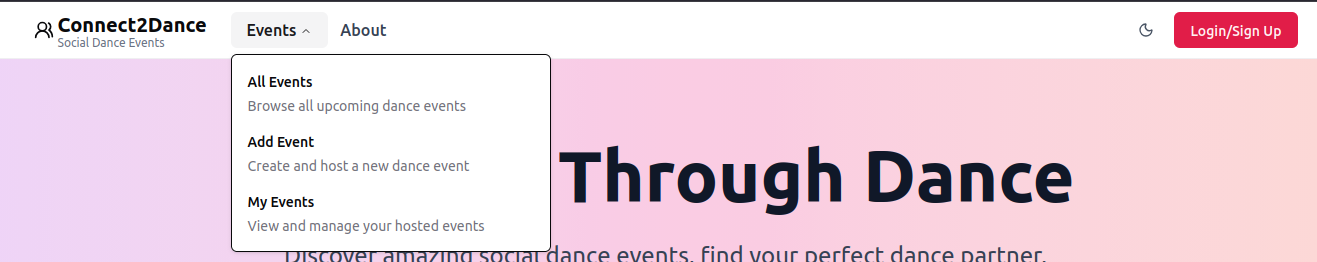
\includegraphics[width=\textwidth]{images/navbar.png}
    \caption{Finální design navigační lišty aplikace}
    \label{fig:navbar}
\end{figure}

\subsection{Domovská stránka}
Domovská stránka bude propagovat celou aplikaci a její hlavní funkce. Bude obsahovat krátký popis toho, co aplikace umí a jaké jsou její hlavní funkce. U nich budou 2 tlačítka, jedno (výraznější) pro přihlášení do aplikace a druhé pro zobrazení nadcházejících akcí. Dále bude obsahovat sekci s top funkcionalitama aplikace, proč by uživatelé měli aplikaci používat. Nakonec se zde budou nacházet 3 akce, které se konají v nejbližší době. Tento návrh jsem tvořila na základě požadavku.

Návrh domovské stránky je znázorněn na obrázku TODO.

% \begin{figure}
%     \centering
%     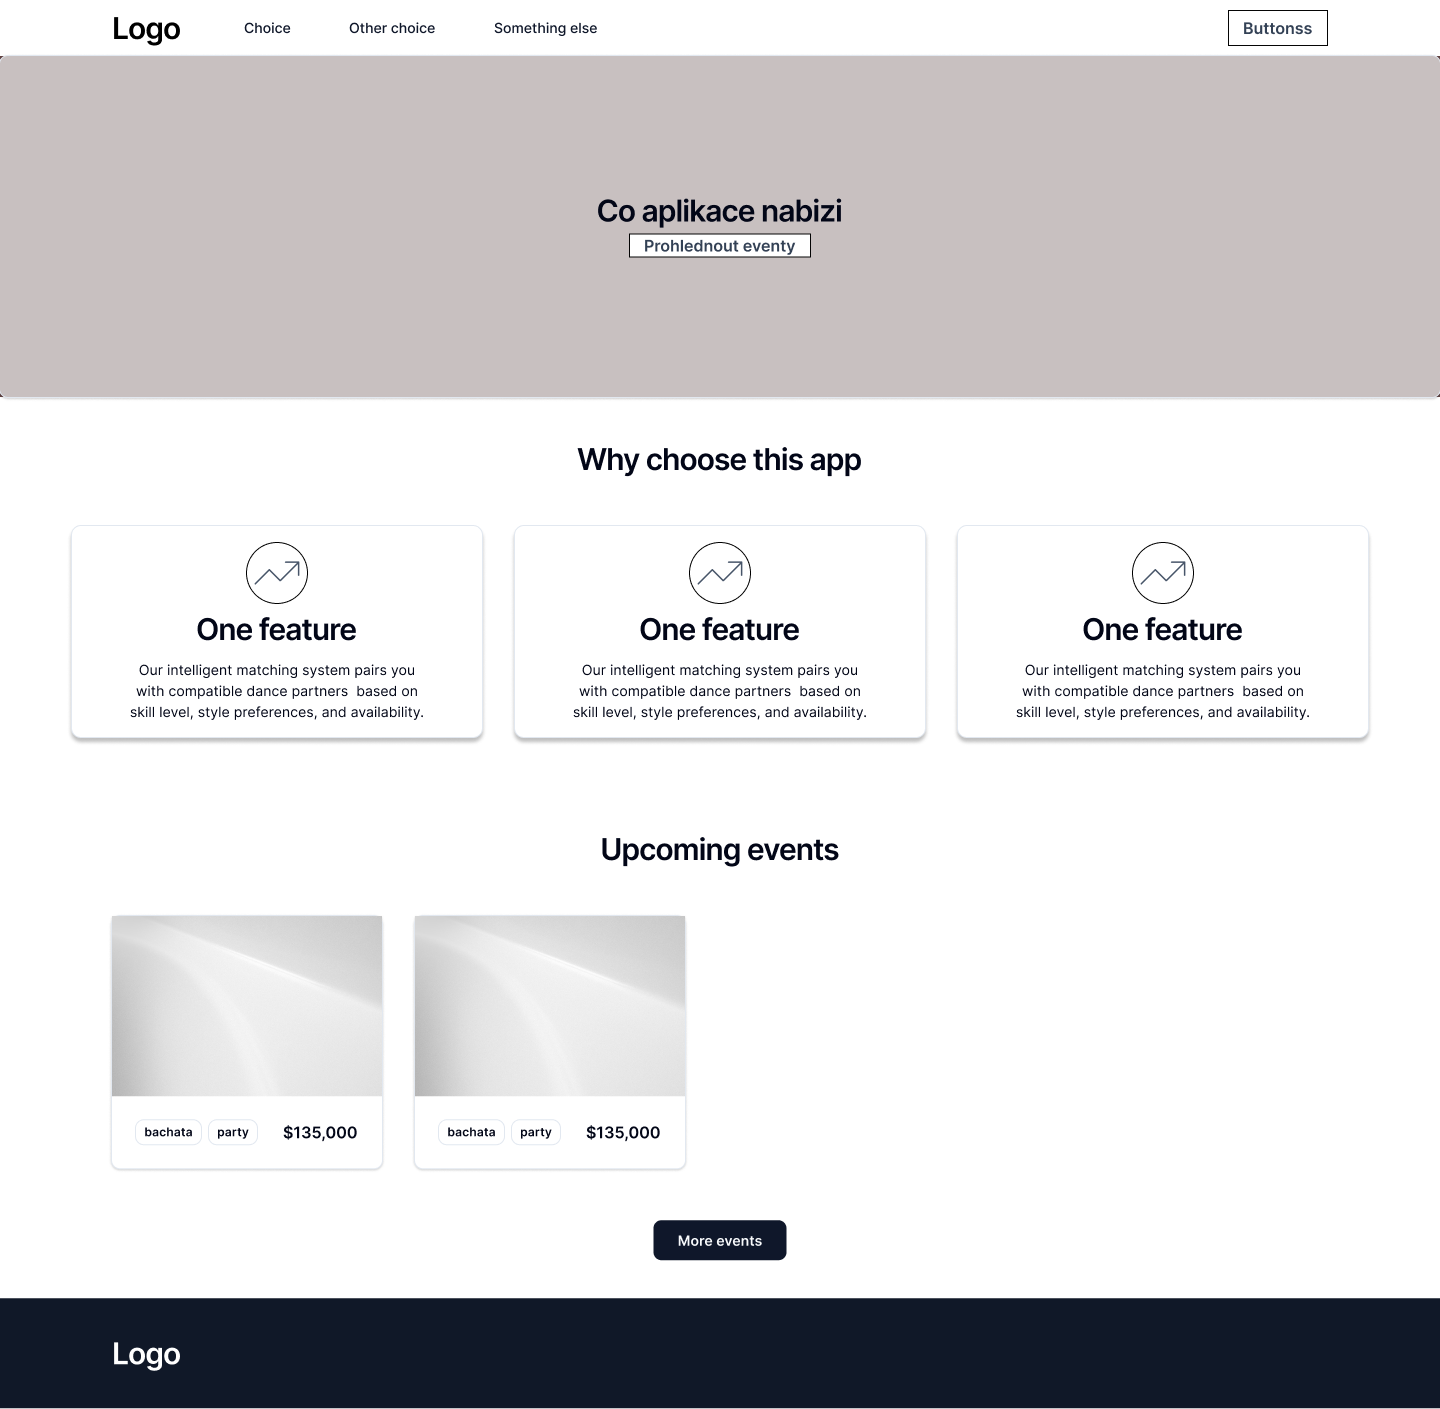
\includegraphics[width=\textwidth]{images/homePage.png}
%     \caption{Návrh domovské stránky}
%     \label{fig:homePage}
% \end{figure}

\subsection{Nadcházející akce}
Tato stránka je velmi důležitá, protože hned po úvodní stránce, je stránkou, kterou uživatelé uvidí a budou se například rozhodovat zda se zaregistrují do aplikace.

Stránka se skládá ze sekce pro vyhledávání akcí a výčtu nadcházejících akcí. Pro vyhledávání jsem navrhla několik inputů, které umožní uživatelům filtrovat akce podle různých kritérií dle požadavku TODO. 

Pro filtrování jména akce jsem se rozhodla navrhnout dlouhý input, následně pro místo konání akce jsem navrhla combobox, který umožní uživatelům potom co začnou psát název místa, zobrazit možnosti, které odpovídají zadanému textu. 

Pro typ akce a typ tance jsem navrhla také comboboxy avšak uživatel může vybrat více možností a pokud je tech možností více než tři tak se zobrazí pouze první tři a zbytek bude zobrazen jako "+X", kde X bude počet zbývajících možností. Po rozkliknutí komboboxu se uživateli zobrazí možnosti které zaškrtl. Tento výběr možností bude na mobilním zařízení implementován tak že vyjede nabídka (podobající se modalu) s možnostmi, které může uživatel zaškrtnout/odškrtnout.

Co se týče zobrazení nadcházejících akcí, navrhla jsem zobrazení ve formě karet, které budou obsahovat informace, jak jsou definované v požadavku TODO. Kartu na desktopovém zařízení jsem pojala tak, že v levé části karty se bude nacházet obrázek akce anebo placeholder pokud obrázek není uvedený. Úplně nahoře v pravé části karty bude název akce, pod ním bude jméno organizátora a následně se budou nacházet zbylé informace o akci, obohacené o ikony. Úplně na spodu karty se budou nacházet akce, když je akce organizována uživatelem, bude se zde nacházet tlačítko přejít na detail akce, pokud uživatel organizátorem není, tak zde navíc budou akce jako přihlásit se na akci a označit že mám zájem o akci. Co mi chvíli dalo zabrat na návrhu bylo umístění tagů, které budou zobrazovat typ akce a typ tance. Nakonec jsem se rozhodla umístit je pod organizátora, kvůli tomu že jsem proiterovala několik variant a tato varianta se uživatelům zdála nejpřehlednější. 

V mobilní variantě se obrázek a informace zobrazí nad sebou, aby se lépe přizpůsobily menší obrazovce.

Základ jsem si nakreslila do figmy, jak mobilní zařízení, tak desktopové zobrazení, ale finální design jsem implementovala rovnou v kódu, protože mi to přišlo efektivnější. Finální design této stránky je znázorněn na obrázku TODO.

\subsection{Detail akce}
Tahle sekce byla pro mě nejtěžší na návrh, protože se zde nachází poměrně hodně informací a akcí, které je potřeba nějak přehledně uspořádat. Při návrhu jsem vycházela z požadavku TODO a také z diskuzí s potenciálními uživateli, kteří mi poskytli cennou zpětnou vazbu ohledně toho, jaké informace by měly být zobrazeny a jak by měly být uspořádány. Při návrhu jsem se inspirovala ze stránech na pořádání událostí jak AllEvents, Eventbrite, Meetup a také z Facebooku, kde se tanečníci nejvíce dozvídají o nadcházejících akcích. Na návrhu této stránky jsem chtěla investovat více času, protože se jedná o jednu z nejklíčovějších stránek celé aplikace a díky této stránce se uživatelé rozhodují, zda se na akci přihlásí, nebo ne. 

Jako první co bude na stránce bude promo obrázek akce, který bude zobrazený v celé šířce stránky. Pokud akce nemá promo obrázek, tak se zobrazí placeholder barva. Na tomto obrázku dole se bude nacházet název akce a pod ním klíčové informace o akci (tyto informace jsou sepsané v požadavku TODO jako základní informace o akci). 

Potom stránka bude obsahovat tlačítka, která umožní pracovat s touto událostí. Tlačítka se liší podle toho zda je uživatel organizátorem akce, přihlášeným uživatelem, nebo uživatelem, který není přihlášený na akci. Pozici tlačítek jsem umístila pod promo obrázek s informacemi o akci, aby byli co nejvíce dostupné a nabádali uživatele k akci. Pokud je uživatel organizátorem akce, bude se zde nacházet tlačítko pro správu akce, které po rozkliknutí nabídne možnosti jako upravit akci a dále podle toho v jakém je akce stavu (smazat/zrušit, publikovat). Pokud uživatel organizátorem není, tak se zobrazují tlačítko pro přihlášení na akci a označení že mám zájem o akci.  

Následně se budou nacházet na stránce tyto sekce (seřazeny od nejdůležitější po nejméně důležitou):
\begin{itemize}
    \item sekce s informacemi o účastnících akce jak je popsáno v požadavku TODO.
    \item popisek akce
    \item detaily akce - zobrazení tagů, které byli popsané v požadavku TODO
    \item sekce s obrázky a videi týkající se akce
    \item sekce s informacemi o organizátorovi akce
\end{itemize}

Zprvu jsem se snažila rozvrhnout jak a kde budou tyto zbývající sekce na stránce. Na mobilním zařízení mi přišlo logické dát jednotlivé sekce dát pod sebou, avšak na větších zařízeních docházelo k tomu, že se stránka stala příliš dlouhou a některé sekce nezabíraly celou šířku stránky, což mi přišlo nevyužité a nehezké z pohledu designu. Nakonec jsem se pro větší zařízení rozhodla pro rozvržení, které je zobrazeno na obrázku TODO, kde se popisek akce a jeho galerie nachází v levé části stránky a zbytek sekcí se nachází v pravé části stránky. Toto rozvržení mi přijde přehlednější a zároveň využívá prostor na stránce lépe než kdybych všechny sekce dala pod sebe. 

Co se týče návrhu jednotlivých sekcí, jejich vytvoření bylo poměrně jednoduché, s výjimkou sekce obsahující informace o účastnících akce. Původně jsem chtěla zobrazovat informace o tom, kolik lidí má o akci zájem a kolik lidí je již registrováno, přičemž jsem se inspirovala zobrazením těchto údajů na Facebooku. Zároveň jsem chtěla zobrazit také kapacitu akce, pokud je definována. Samotné zobrazení těchto údajů nebylo příliš složité, větší výzvou však bylo navrhnout způsob prezentace zastoupení jednotlivých rolí v případě akcí, které evidují rozdělení účastníků podle rolí.

Nakonec jsem zvolila design ve formě karty, která zobrazuje počet registrovaných účastníků a počet lidí, kteří o akci projevili zájem. Pokud má akce omezenou kapacitu, zobrazuje se zde také informace o počtu zbývajících míst, která je vizuálně reprezentována pomocí progress baru (viz karta Who's Coming na obrázku \ref{fig:eventDetail}).

V případě, že je u akce evidováno rozdělení účastníků podle rolí, karta navíc zobrazuje také jejich zastoupení. Jednotlivé role jsou uvedeny pod sebou v samostatných řádcích, kde je uveden název role a počet účastníků v dané roli. I zde je použit progress bar, který znázorňuje poměr zastoupení jednotlivých rolí, případně reflektuje celkovou kapacitu akce, pokud je stanovena.

Pokud akce nemá definovanou kapacitu a zároveň se při registraci nerozlišují role, zobrazuje se pouze počet registrovaných účastníků a počet lidí, kteří o akci projevili zájem.

Dále jsem chtěla uživatelům umožnit zobrazit konkrétní účastníky akce. Proto jsem navrhla, aby po kliknutí na tuto kartu došlo k otevření modálního okna se seznamem účastníků. Pokud je při registraci uváděna také role, modal rozdělí účastníky do samostatných sekcí podle jednotlivých rolí. V opačném případě se zobrazí pouze jeden seznam všech účastníků.

Sekce týkající se detailů akce a organizátora jsem navrhla také ve formě karet, aby byl celkový design stránky vizuálně konzistentní.

Sekce galerie obsahuje náhledy obrázků a videí, které jsou zobrazeny ve formě karet. Po kliknutí na konkrétní médium se obsah zobrazí v plné velikosti a v případě videa se zároveň spustí jeho přehrávání.

\begin{figure}
    \centering
    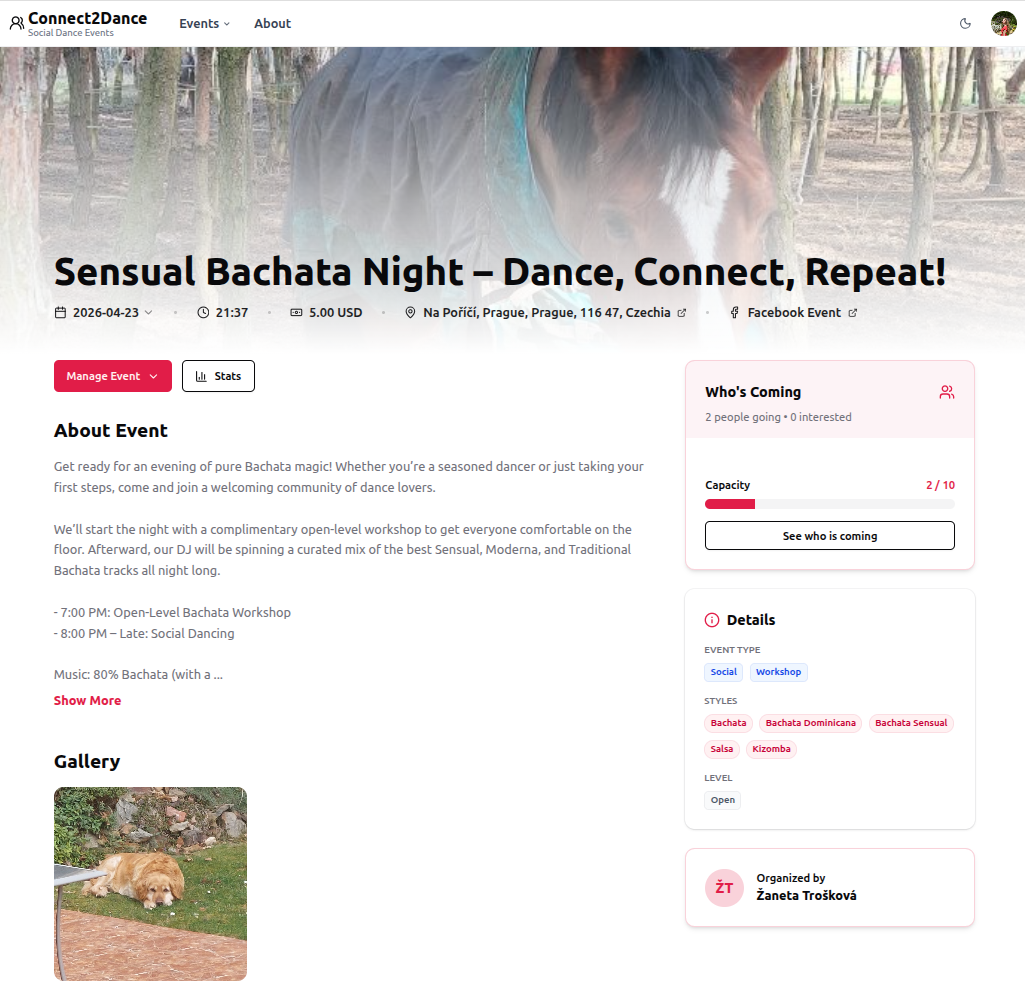
\includegraphics[width=\textwidth]{images/event-detail.png}
    \caption{Finální design detailu akce}
    \label{fig:eventDetail}
\end{figure}

\subsection{Modal na publikování akce}
Obvykle modály na jednoduché akce jako např. smazání události nejsou třeba speciálně navrhovat. V případě publikace akce se, ale jedná o modal obsahující formulář, ze kterého uživatel vybírá jak chce publikovat akci. Způsoby publikace akce jsou popsány v požadavku TODO. Proto jsem se rozhodla tento modal navrhnout, aby bylo jasné, jak bude vypadat a jak bude fungovat. Modal obsahuje název "Publish event", krátký popis toho, co zveřejnění akce znamená a co se stane po zveřejnění, a dále obsahuje formulář s možností výběru způsobu zveřejnění akce. Pro všechny druhy publikace akce existuje možnost zda uživatel chce potvrzovat jednotlivé registrace uživatelů či ne.

\subsection{Profil uživatele}
Profil uživatele jsem se snažila navrhnout tak, aby byl přehledný a obsahoval důležité informace o uživateli. Zároveň jsem chtěla aby designem evokoval profil na sociální síti, protože jsou uživatelé na takové rozhraní zvyklí a bude pro ně přirozené se v něm pohybovat. Profil uživatele se skládá z dvou částí:
\begin{itemize}
    \item karta s informacemi o uživateli, která obsahuje informace jako jméno a příjmení uživatele, hlavní role v tanci(leader, follower, role rotation), avatar uživatele, obecná úroveň v tanci, popis o sobě a taneční styly, které uživatel tancuje. Pokud je profil přihlášeného uživatele, tak se zde navíc nachází tlačítko pro úpravu profilu.
    \item galerie s obrázky a videi, které uživatel přidal do svého profilu. Galerie je řešena stejným designem jako u detailu akce.
\end{itemize}
Informace o tom co zobrazit v profilu uživatele jsem navrhla na základě požadavku TODO a galerii jsem navrhla na základě požadavku TODO.

Pokud jde o upravování profilu, tak po kliknutí na tlačítko pro úpravu profilu se zobrazí formulář, který umožní uživateli upravit informace na profilu. Sekce galerie se v v tomto případě přesune do karty s formulářem, kde uživatel může přidat nové obrázky a videa, nebo odstranit stávající.

Výsledný design profilu uživatele je znázorněn na obrázku \ref{fig:userProfile}.

\begin{figure}
    \centering
    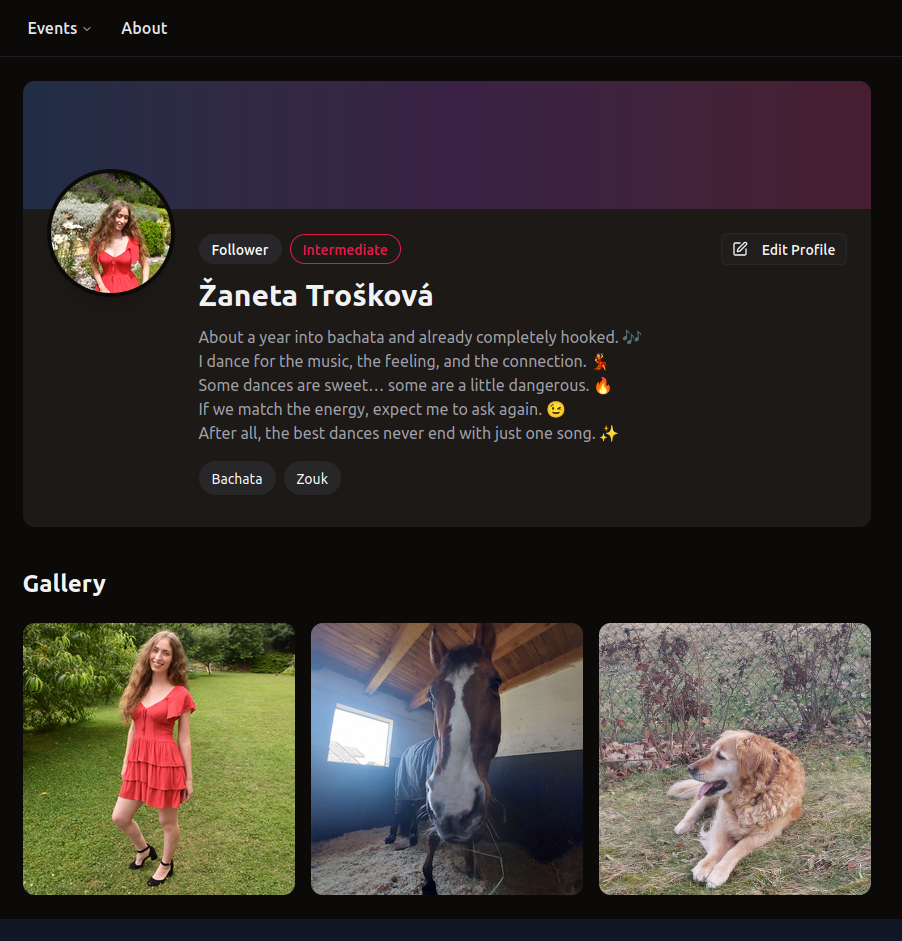
\includegraphics[width=\textwidth]{images/profile.png}
    \caption{Výsledný profil uživatele}
    \label{fig:userProfile}
\end{figure}

\subsection{Moje akce}
Tato stránka bude obsahovat seznamy akcí, které uživatel organizuje, na které se přihlásil a které označil že ho zajímají na základě požadavku TODO. Jelikož se jedná o seznamy, které jsou vzájemně disjunktní, navrhla jsem zobrazení pomocí komponenty Tabs, která umožní uživateli přepínat mezi jednotlivými seznamy. Zároveň se bude naho5e objevovat tlačítko pro vytvoření nové akce a nadpis "My events".

Pokud se jedná o akci, která je opakovaná, tak se zobrazí název celé této série s rozsahem datumů od první do poslední akce, a pod tím se zobrazí pomocí tabulky jednotlivé výskyty této akce. Tabulka obsahuje datum a čas konání výskytu, místo konání, počet přihlášených uživatelů a status akce, popřípadě status uživatele, pokud jsme v sekci přihlášených akcí. Také se pro každý výskyt nachází tlačítko pro zobrazení detailu výskytu, které přesměruje uživatele na detail výskytu akce. 

Pokud se jedná o akci, která není opakovaná, tak se zobrazí karta s názvem akce, datem a časem konání, místem konání, počtem přihlášených uživatelů a počtem uživatelů, kteří označili že je akce zajímá, a status akce, popřípadě status uživatele, pokud jsme v sekci přihlášených akcí. Také je zde tlačítko pro zobrazení detailu akce, které přesměruje uživatele na detail akce. 

Přemýšlela jsem nad tím, že minimálně v případě jednorázové akce bych nemusela implementovat tlačítko pro zobrazení detailu akce, ale místo toho by se uživatel mohl dostat na detail akce kliknutím na kartu s informacemi o akci. Nakonec jsem se však rozhodla implementovat tlačítko pro zobrazení detailu akce, protože mi přijde přehlednější a zároveň je to konzistentní s tím, jak je to v případě opakovaných akcí.

Pokud uživatel nemá žádné akce v dané sekci, tak se zobrazí karta s informací, že v této sekci nejsou žádné akce a s výzvou k tomu, aby uživatel začal procházet nadcházející akce a přihlásil se na nějakou z nich, nebo začal organizovat vlastní akci.

Na obrázku \ref{fig:myEvents} je znázorněna finální implementace této stránky v sekci událostí, které uživatel organizuje. Obrázek ukazuje, jak se zobrazí opakovaná akce, která má více výskytů, a také zobrazení jednorázové akce.

\begin{figure}
    \centering
    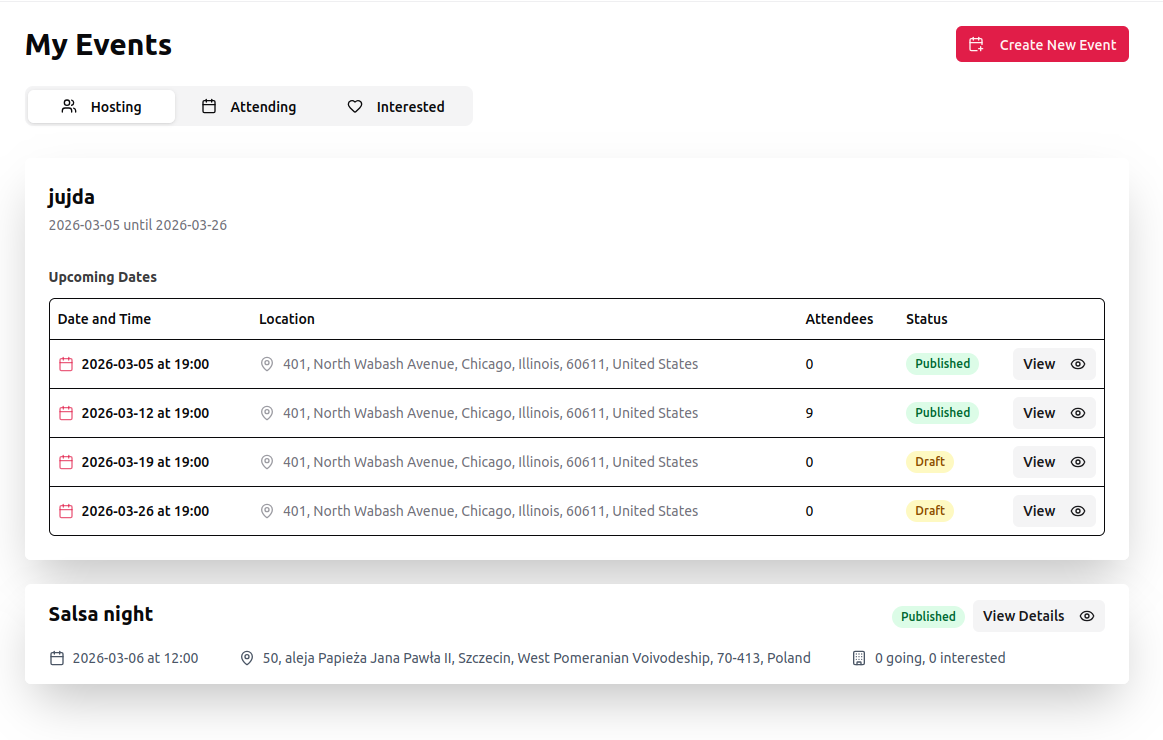
\includegraphics[width=\textwidth]{images/my-events.png}
    \caption{Finální implementace stránky "Moje akce"}
    \label{fig:myEvents}
\end{figure}

\subsection{Vytvořit akci}
Tuto část aplikace jsem navrhovala na základě požadavku TODO, který obsahuje informace o tom, jaké informace by měl formulář pro vytvoření akce obsahovat. 

Prvně jsem přemýšlela nad tím zda nemít jeden velký jednostránkový formulář. Toto řešení jsem navrhla protože z požadavku vyplívá, že pro vytvoření akce je potřeba zadat poměrně hodně informací, a já nechci aby se uživatelům zobrazoval příliš dlouhý formulář, který by je mohl odradit od vytvoření akce. Chvíli jsem ještě přemýšlela, že by sekce byly ve sbalitelných sekcích, což by mohlo napomoct k pocitu uživatele, že formulář není tak dlouhý. Avšak nakonec jsem se rozhodla rozdělit formulář do několika kroků, protože mi přijde přehlednější a mohu informace rozdělit do logických celků, což může uživatelům pomoci lépe se orientovat v tom, co mají zadat a zároveň se nemusí cítit zahlcení množstvím informací, které musí zadat najednou.

Existuje spousty způsobů, jak koncipovat aby každá sekce měla jednu stránku a mezi nimi se dalo přepínat. Pro inspiraci jsem procházela různé weby zaobírající se organizací akcí, jako například AllEvents. Na této stránce se používá pro přecházení mezi jednotlivými sekcemi formuláře boční nabídka. Toto řešení se mi moc nelíbí, protože mi přijde, že zbytečně zabírá místo na obrazovce a zároveň ve zbytku aplikace nepoužívám žádné boční menu, takže by to bylo nekonzistentní. 

Nakonec jsem se rozhodla pro řešení, které bude obsahovat kartu s jednotlivými kroky formuláře, která bude umístěna v levé části obrazovky a bude obsahovat název každého kroku a indikátor toho, který krok je aktuálně zobrazený. Po kliknutí na název kroku se uživatel přepne na tento krok. Toto řešení se mi líbí, protože je přehledné a uživatel je provázen celým procesem vytváření akce. Jediná nevýhoda tohoto řešení je, že zabírá místo na obrazovce, což na mobilních zařízeních může být problém. Proto jsem pro mobilní zobrazení navrhla, aby se místo karty s kroky zobrazoval pouze název aktuálního kroku a progres bar, který bude indikovat, kolik kroků uživatel již prošel a kolik jich ještě zbývá. V obou případech se budou tlačítka na přechod mezi jednotlivými kroky nacházet v dolní části obrazovky. Na posledním kroku se místo tlačítka pro přechod na další krok bude nacházet tlačítko pro odeslání formuláře a vytvoření akce.

Dalším krokem bylo jak rozdělit informace do jednotlivých kroků. Jelikož je informací poměrně hodně i v rámci jednoho kroku, tak jsem se snažila informace rozdělit do logických celků, které spolu souvisí.

Dospěla jsem k následujícímu rozdělení:
\begin{itemize}
    \item krok 1 - základní informace o akci
    \begin{itemize}
        \item základní informace o akci (jméno akce, lokace)
        \item datum a čas konání akce - v případě jednorázové lze navíc doplnit datum konce akce, v případě opakované akce datum posledního výskytu akce a frekvence opakování akce (denně, týdně, měsíčně)
        \item cena - kolik akce stojí a jaká je měna
    \end{itemize}
    \item krok 2 - popis akce - zvolila jsem proto tento prvek samostatný krok, protože z mých zkušeností bývá velmi dlouhý.
    \item krok 3 - média týkající se akce (zvolit primární obrázek akce, který se bude zobrazovat v přehledu nadcházejících akcí, a další obrázky a videa týkající se akce)
    \item krok 4 - doplňující informace o akci
    \begin{itemize}
        \item doplňující informace o akci (typ akce, typ tance, pro jakou úroveň tanečníků je akce určena, odkaz na facebookovou událost akce)
        \item informace ke kapacitě akce (maximální počet účastníků)
    \end{itemize}
\end{itemize}

\subsection{O aplikaci}
Tato stránka nebyla potřeba nijak vzlášť navrhovat, protože bude obsahovat pouze textové informace o aplikaci, které budou rozděleny do několika odstavců. 
Stránka bude obsahovat informace z požadavku TODO.

\subsection{Stránka s registrovanými uživateli}
Tato stránka bude přístupná pouze pro organizátory dané akce a bude obsahovat seznam všech registrací pro danou událost a možnosti s registrací pracovat (například zrušit registraci, přijmout registraci, atd.). 

Stránka bude tvořena názvem akce a pod ním bude datum akce. V případě že je akce opakovaná, bude zde stejná komponenta jako u detailu akce, která dovolí přepínat mezi jednotlivými výskyty akce.

Pod tím se bude nacházet tabulka, která bude obsahovat informace o registracích pro danou akci. Hlavička tabulky bude obsahovat zaškrtávací pole pro označení všech registrací, informace o uživateli, který se registroval, datum registrace a status registrace. 
Při zaškrtnutí konkrétní registrace se zobrazí možnosti pro práci s touto registrací, například zrušení registrace, přijetí registrace, atd. Každá hlavička tabulky obsahuje vhodný filtr pro každý sloupec, což může umožnit například filtrovat registrace podle statusu registrace, který organizátor chce vidět.

\subsection{Přihlašování a odhlašování z aplikace}
Pro přihlašování do aplikace jsem navrhla samostatnou stránku, která obsahuje kartu s tlačítkem umožňujícím přihlášení pomocí účtu Google. V případě potřeby rozšíření o další způsoby přihlašování, například pomocí e-mailu a hesla, by bylo možné tyto možnosti do stejné karty snadno doplnit.

Pokud se uživatel rozhodne z aplikace odhlásit, je po provedení této akce přesměrován na stránku s informací, že odhlášení proběhlo úspěšně. Tlačítko pro opětovné přihlášení jsem na tuto stránku záměrně neumísťovala, protože možnost přihlášení je již dostupná v navigační liště aplikace.









\chapter{Implementace}

\section{Server}
\subsection{API na lokace}
Při tvorbě taneční akce je potřeba zadat lokaci, kde se bude konat. Jelikož nechci aby uživatelé zadávali lokaci ručně (jue to nepohodlné a může to vést k chybám), bylo potřeba najít správné API, které umožňuje získávat lokace zadané uživatelem. Zároveň ale pořád chci umožnit lokaci ručně upravit, protože je možné, že některé lokace budou v API chybět (například se bude v API nacházet ulice, ale ne s číslem popisným, na které se akce bude konat). V následujících odstavcích popíšu, mezi jakými API jsem vybírala a která byla nakonec zvolena.

\subsubsection{Google places API (New)}
Jedná se o vystavenou službu od společnosti Google, která umožňuje pracovat s lokacemi. Toto API nabízí širokou škálu funkcí \cite{google_places_api_overview} jako například: 
\begin{itemize}
    \item Place Details (New) - API umožňuje získat podrobné informace o konkrétním místě, jako je adresa, telefonní číslo, hodnocení, fotografie a další.
    \item Text Search (New) - API umožňuje hledat místa na základě textového dotazu, jako je název místa, adresa nebo kategorie.
    \item Nearby Search (New) - API umožňuje hledat místa v okolí zadaných geografických souřadnic.
    \item Autocomplete (New) - API umožňuje získat návrhy míst na základě částečného textového dotazu a geografického rozsahu.
\end{itemize} 
S tímto API jsem se již setkala v několika aplikacích při zadávání lokace pro události (například v aplikaci OnlyDance).

Toto API jsem nakonec nezvolila, kvůli tomu, že je placené a cena se odvíjí od počtu požadavků, které jsou na API posílány. Jelikož nechci aby projekt se stal finančně náročným, rozhodla jsem podívat se po nějaké levnější alternativě, která by mi poskytla podobné funkce.\cite{google_maps_places_pricing}

\subsubsection{Photon (https://github.com/komoot/photon)}
Toto API je open-source a je založeno na OpenStreetMap datech. API nabízí funkce jako například:
\begin{itemize}
    \item Geocoding
    \item Reverse Geocoding
    \item hledání míst - podporuje i v rámci několika jazyků
\end{itemize}
Tento projekt má i vystavené zdarma API, které je možné využívat bez nutnosti hostovat vlastní instanci. Avšak je třeba dbát na to nezahlcovat toto API přílišným množstvím požadavků, protože na to server není připraven a jedná se spíše o ukázku toho, jak API funguje. Pokud by bylo třeba posílat větší množství požadavků, tak je v projektu zdokumentováno jak hostovat vlastní instanci. \cite{komoot_photon}

Nakonec jsem se rozhodla pro využití tohoto API, protože je zdarma a poskytuje všechny funkce, které potřebuji pro zadávání lokace pro události. Jelikož moje aplikace je ve fázi prototypu, nebude na API posíláno příliš mnoho požadavků, takže by neměl být problém s využíváním tohoto API. V budoucnu, pokud by se aplikace stala populární a bylo by potřeba posílat větší množství požadavků, bych zvážila hostování vlastní instance tohoto API nebo přechod na placené API, jako je Google Places API. Navíc při zadávání lokace bude nastavený přiměřený \textit{debounce}, aby se zabránilo posílání příliš mnoha požadavků na API.

\subsection{Přihlášení uživatele}
Přihlášení uživatele jak již bylo zmíněno v předchozí kapitole, bylo realizováno pomocí Google. Jelikož naše aplikace není jen klientská, ale i serverová, bylo potřeba implementovat přihlášení i na serveru.

Prvním krokem bylo vytvoření projektu v Google Cloud Console, Poté bylo potřeba vytvořit OAuth 2.0 Client ID pro webovou aplikaci, což nám poskytlo Client ID a Client Secret, které jsou nezbytné pro implementaci přihlášení. Následně byly nastaveny redirect URI, které jsou adresy, na které bude Google přesměrovávat uživatele po úspěšném přihlášení a origins, které jsou adresy, ze kterých bude možné přihlášení provést.

Poté byly přidány tzv. scopes, které určují, jaké informace o uživateli bude aplikace požadovat. V našem případě bude při prvotním přihlášení požadováno pouze základní informace o uživateli, jako je jeho jméno a emailová adresa. Tudíž se jedná o následující scopes \cite{google_oauth_scopes}:
\begin{itemize}
    \item \texttt{openid} - Tento scope propojuje uživatele s jeho osobními údaji na Google účtu.
    \item \texttt{profile} - Tento scope umožňuje získat osobní údaje uživatele, i které zveřejnil
    \item \texttt{email} - Tento scope umožňuje získat primární emailovou adresu uživatele.
\end{itemize} 

Tyto scope se řadí mezi nesenzitivní oprávnění, což jsou oprávnění, která slouží k autorizaci uživatele. 
\cite{google_drive_auth_guide}

Při nasazení aplikace do produkce a využívání api google, google nevyžaduje u těchto oprávnění ověření. Tudíž je jednodušší aplikaci uvést do produkce. 
\cite{google_app_verification}

\subsubsection{Inkrementální autorizace}
Aplikace bude kromě zmíněných oprávněních z předešlé sekce také vyžadovat oprávnění pro přístup k Google Forms API, aby uživatelé mohli propojit formulář a odpovědi z formuláře s aplikací. Oprávnění jsou následující \cite{google_oauth_scopes}:
\begin{itemize}
    \item \texttt{https://www.googleapis.com/auth/forms.body} - Tento scope umožňuje aplikaci číst a upravovat obsah formulářů, jako jsou otázky,
    \item \texttt{https://www.googleapis.com/auth/forms.responses.readonly} - Tento scope umožňuje aplikaci číst odpovědi z formulářů, ale neumožňuje je upravovat.
\end{itemize}

Jelikož se může stát že uživatel nebude nikdy potřebovat propojit formulář s aplikací, bylo by zbytečné požadovat tato oprávnění již při prvotním přihlášení. Proto je implementována tzv. inkrementální autorizace, která umožňuje požádat o další oprávnění až v momentě, kdy jsou potřeba. V našem případě se tedy o tato oprávnění požádá až v momentě, kdy se uživatel bude snažit propojit formulář s aplikací. Pokud uživatel tato oprávnění již udělil, nebude o ně požádán znovu. \cite{google_oauth_incremental_auth}

Obecně inkrementální autorizace funguje tak, že uživatel požádá o oprávnění, která potřebuje a endpoint Google vrátí kód, který dále může být vyměněn za access token obsahující všechny oprávnění, která uživatel udělil. Tento způsob je od Google považován jako doporučený, oproti například požádání všech oprávnění najednou. \cite{google_oauth_incremental_auth} 

\subsubsection{Proces přihlášení}
Proces přihlášení začína na straně klienta. Uživatel klikne na tlačítko Sign in a klient provolá api Google pro přihlášení.

Url, které klient volá pro přihlášení, je následující \cite{google_oauth_scopes}:

\begin{lstlisting}[language=TypeScript]
export const buildGoogleOAuthUrl = (params: {
  scope: string;
  state?: string;
}) => {
  const baseUrl = GOOGLE_OAUTH_URL;
  const urlParams = new URLSearchParams({
    client_id: GOOGLE_CLIENT_ID,
    redirect_uri: GOOGLE_REDIRECT_URI,
    response_type: 'code',
    scope: params.scope,
    access_type: 'offline',
    include_granted_scopes: true.toString()
  });

  if (params.state) {
    urlParams.append('state', params.state);
  }

  return `${baseUrl}?${urlParams.toString()}`;
};
\end{lstlisting}

Funkci jsem si naprogramovala sama i přes to, že existuje například knihovna \texttt{@react-oauth/google}, která zjednodušuje proces přihlášení. Avšak při implementaci jsem narazila na problém, že tato knihovna v případě že využíváme flow autorization code, automaticky posílá parameter prompt=consent, což způsobuje, že uživatel musí při každém přihlášení proklikat souhlas s oprávněními, i když je již udělil. Tudíž jsem se rozhodla implementovat přihlášení sama, abych měla plnou kontrolu nad tím, jaké parametry jsou posílány a mohla tak využít inkrementální autorizaci.

Parametry, které jsou posílány v url pro přihlášení, jsou následující \cite{google_oauth_creating_client}:
\begin{itemize}
    \item \texttt{client\_id} - Toto je Client ID, které jsme získali při vytvoření OAuth 2.0 Client ID v Google Cloud Console.
    \item \texttt{redirect\_uri} - Toto je URI, na které bude Google přesměrovávat uživatele po úspěšném přihlášení. Toto URI musí být stejné jako jedno z redirect URI, které jsme nastavili v Google Cloud Console.
    \item \texttt{response\_type} - Tento parameter určuje, jaký typ odpovědi očekáváme od Google. V našem případě je to \texttt{code}, což znamená, že očekáváme autorizační kód, který následně vyměníme za access token. Druhým typem odpovědi je \texttt{token}, což znamená, že očekáváme přímo access token. Tento typ odpovědi se používá v tzv. implicitním flow, které se však nedoporučuje pro webové aplikace, protože není tak bezpečné jako authorization code flow.
    \item \texttt{scope} - Tento parameter obsahuje seznam oprávnění, o která žádáme. Oprávnění jsou oddělena mezery.
    \item \texttt{access\_type} - Tento parameter určuje, zda chceme získat refresh token. Pokud je tento parameter nastaven na \texttt{offline}, Google nám pošle refresh token, který můžeme použít k získání nového access tokenu, když ten původní vyprší. Parametr jsem takto zvolila kvůli tomu, že bude vyžadováno abychom v budoucnu volali API i bez přítomnosti uživatele, například pro synchronizaci odpovědí z formuláře, a v takovém případě je potřeba mít možnost získat nový access token bez toho, aby se uživatel musel znovu přihlásit.
    \item \texttt{include\_granted\_scopes} - Tento parameter určuje, zda chceme, aby Google zahrnul již udělená oprávnění do access tokenu. Pokud je tento parameter nastaven na \texttt{true}, Google nám pošle access token, který obsahuje všechna oprávnění, která uživatel udělil, nejen ta, o která právě žádáme. Při implementaci se mi stalo, že jsem na tento parametr opomněla a v důsledku při každém přihlášení uživatel resetoval všechna oprávnění, která udělil, a musel je znovu udělovat, což samozřejmě nebylo ideální.
    \item \texttt{state} - Tento parameter je volitelnný a slouží k ochraně proti CSRF útokům. Můžeme do něj vložit náhodný řetězec, který nám Google vrátí zpět po úspěšném přihlášení. Tím můžeme ověřit, že odpověď pochází od Google a ne od útočníka.
\end{itemize}

Potom co uživatel zvolí účet, kterým se chce přihlásit, a udělí požadovaná oprávnění (pokud je ještě neudělil), Google přesměruje uživatele na redirect URI, které jsme nastavili, a v URL bude obsažen autorizační kód. Klient tento kód zachytí a pošle ho na náš server, kde ho vyměníme za access token. Pokud se jedná o prvotní přihlášení, Google nám pošle i refresh token, který uložíme do databáze pro pozdější použití. Poté obratem klientovi vrátíme serverem vygenerovaný JWT token, který klient bude používat pro autentizaci a autorizaci při dalších požadavcích na server.


\subsection{Integrace s Google Forms}
\section{Frontend}
\section{Databáze}
\chapter{Testování}
\begin{chapterabstract}
Tato kapitola popisuje testování aplikace. Nejprve jsou zadefinovány pojmy týkající se testování. Poté je uvedeno jakým způsobem bylo testování funkcionalit systému prováděno a proč bylo zvolen zrovna tento způsob testování. Závěrečná část kapitoli se věnuje uživatelskému testování, jenž bylo prováděno s potencionálními uživateli aplikace. Nakonec jsou uvedeny výsledky testování a závěry, které z nich byly vyvozeny.
\end{chapterabstract}

\section{Testování}

 % include `text.tex' from `text/' subdirectory

\appendix\appendixinit % do not remove these two commands

\include{text/appendix} % include `appendix.tex' from `text/' subdirectory

\backmatter % do not remove this command

\printbibliography % print out the BibLaTeX-generated bibliography list

\chapter{Obsah příloh}
% Contents of the attachment

	\dirtree{%
		.1 /.
		.2 readme.txt\DTcomment{stručný popis obsahu média}.
		.2 src.
		.3 impl\DTcomment{zdrojové kódy implementace}.
		.4 be-dance-app\DTcomment{zdrojové kódy implementace backendové části}.
		.4 fe-dance-app\DTcomment{zdrojové kódy implementace frontendové části}.
		.3 thesis\DTcomment{zdrojová forma práce ve formátu \LaTeX{}}.
		.2 text\DTcomment{text práce}.
		.3 thesis.pdf\DTcomment{text práce ve formátu PDF}.
	}
 % include `medium.tex' from `text/' subdirectory

\end{document}
